\documentclass[12pt,a4paper]{article}
\usepackage{hyperref}
\usepackage{graphicx}
\begin{document}
\begin{titlepage}
	\centering
	
\includegraphics[width=0.15\textwidth]{cern}\hspace{50mm}

\includegraphics[width=0.15\textwidth]{Alpha}	
	
	\par\vspace{1cm}
	{\scshape\LARGE CERN Summer Program Report 2019\footnote{You can find all of the documents of my projects on CERN repository in my Github page: \url{https://github.com/alifele/My_Poroject_at_CERN}} \par}
	\vspace{1cm}
	
	\vspace{1.5cm}
	
	\vspace{2cm}
	\begin{Large}
	Author:
	\end{Large} \par
	{\Large\itshape Ali Fele Paranj \par}
	\vspace{30mm}
	supervised by\par
	Dr. Muhammed Sameed
	\vfill
% Bottom of the page
	{\large \today\par}

\end{titlepage}



\newpage

\tableofcontents

\newpage

\section{How ALPHA Works}

ALPHA is an international  collaboration based at CERN, which is working with trapped antihydrogen atoms, the antimatter counterpart of the simplest atom, hydrogen. By precise comparisons of hydrogen and antihydrogen, the experiment hopes to study fundamental symmetries between matter and antimatter. 

\begin{figure}[h]

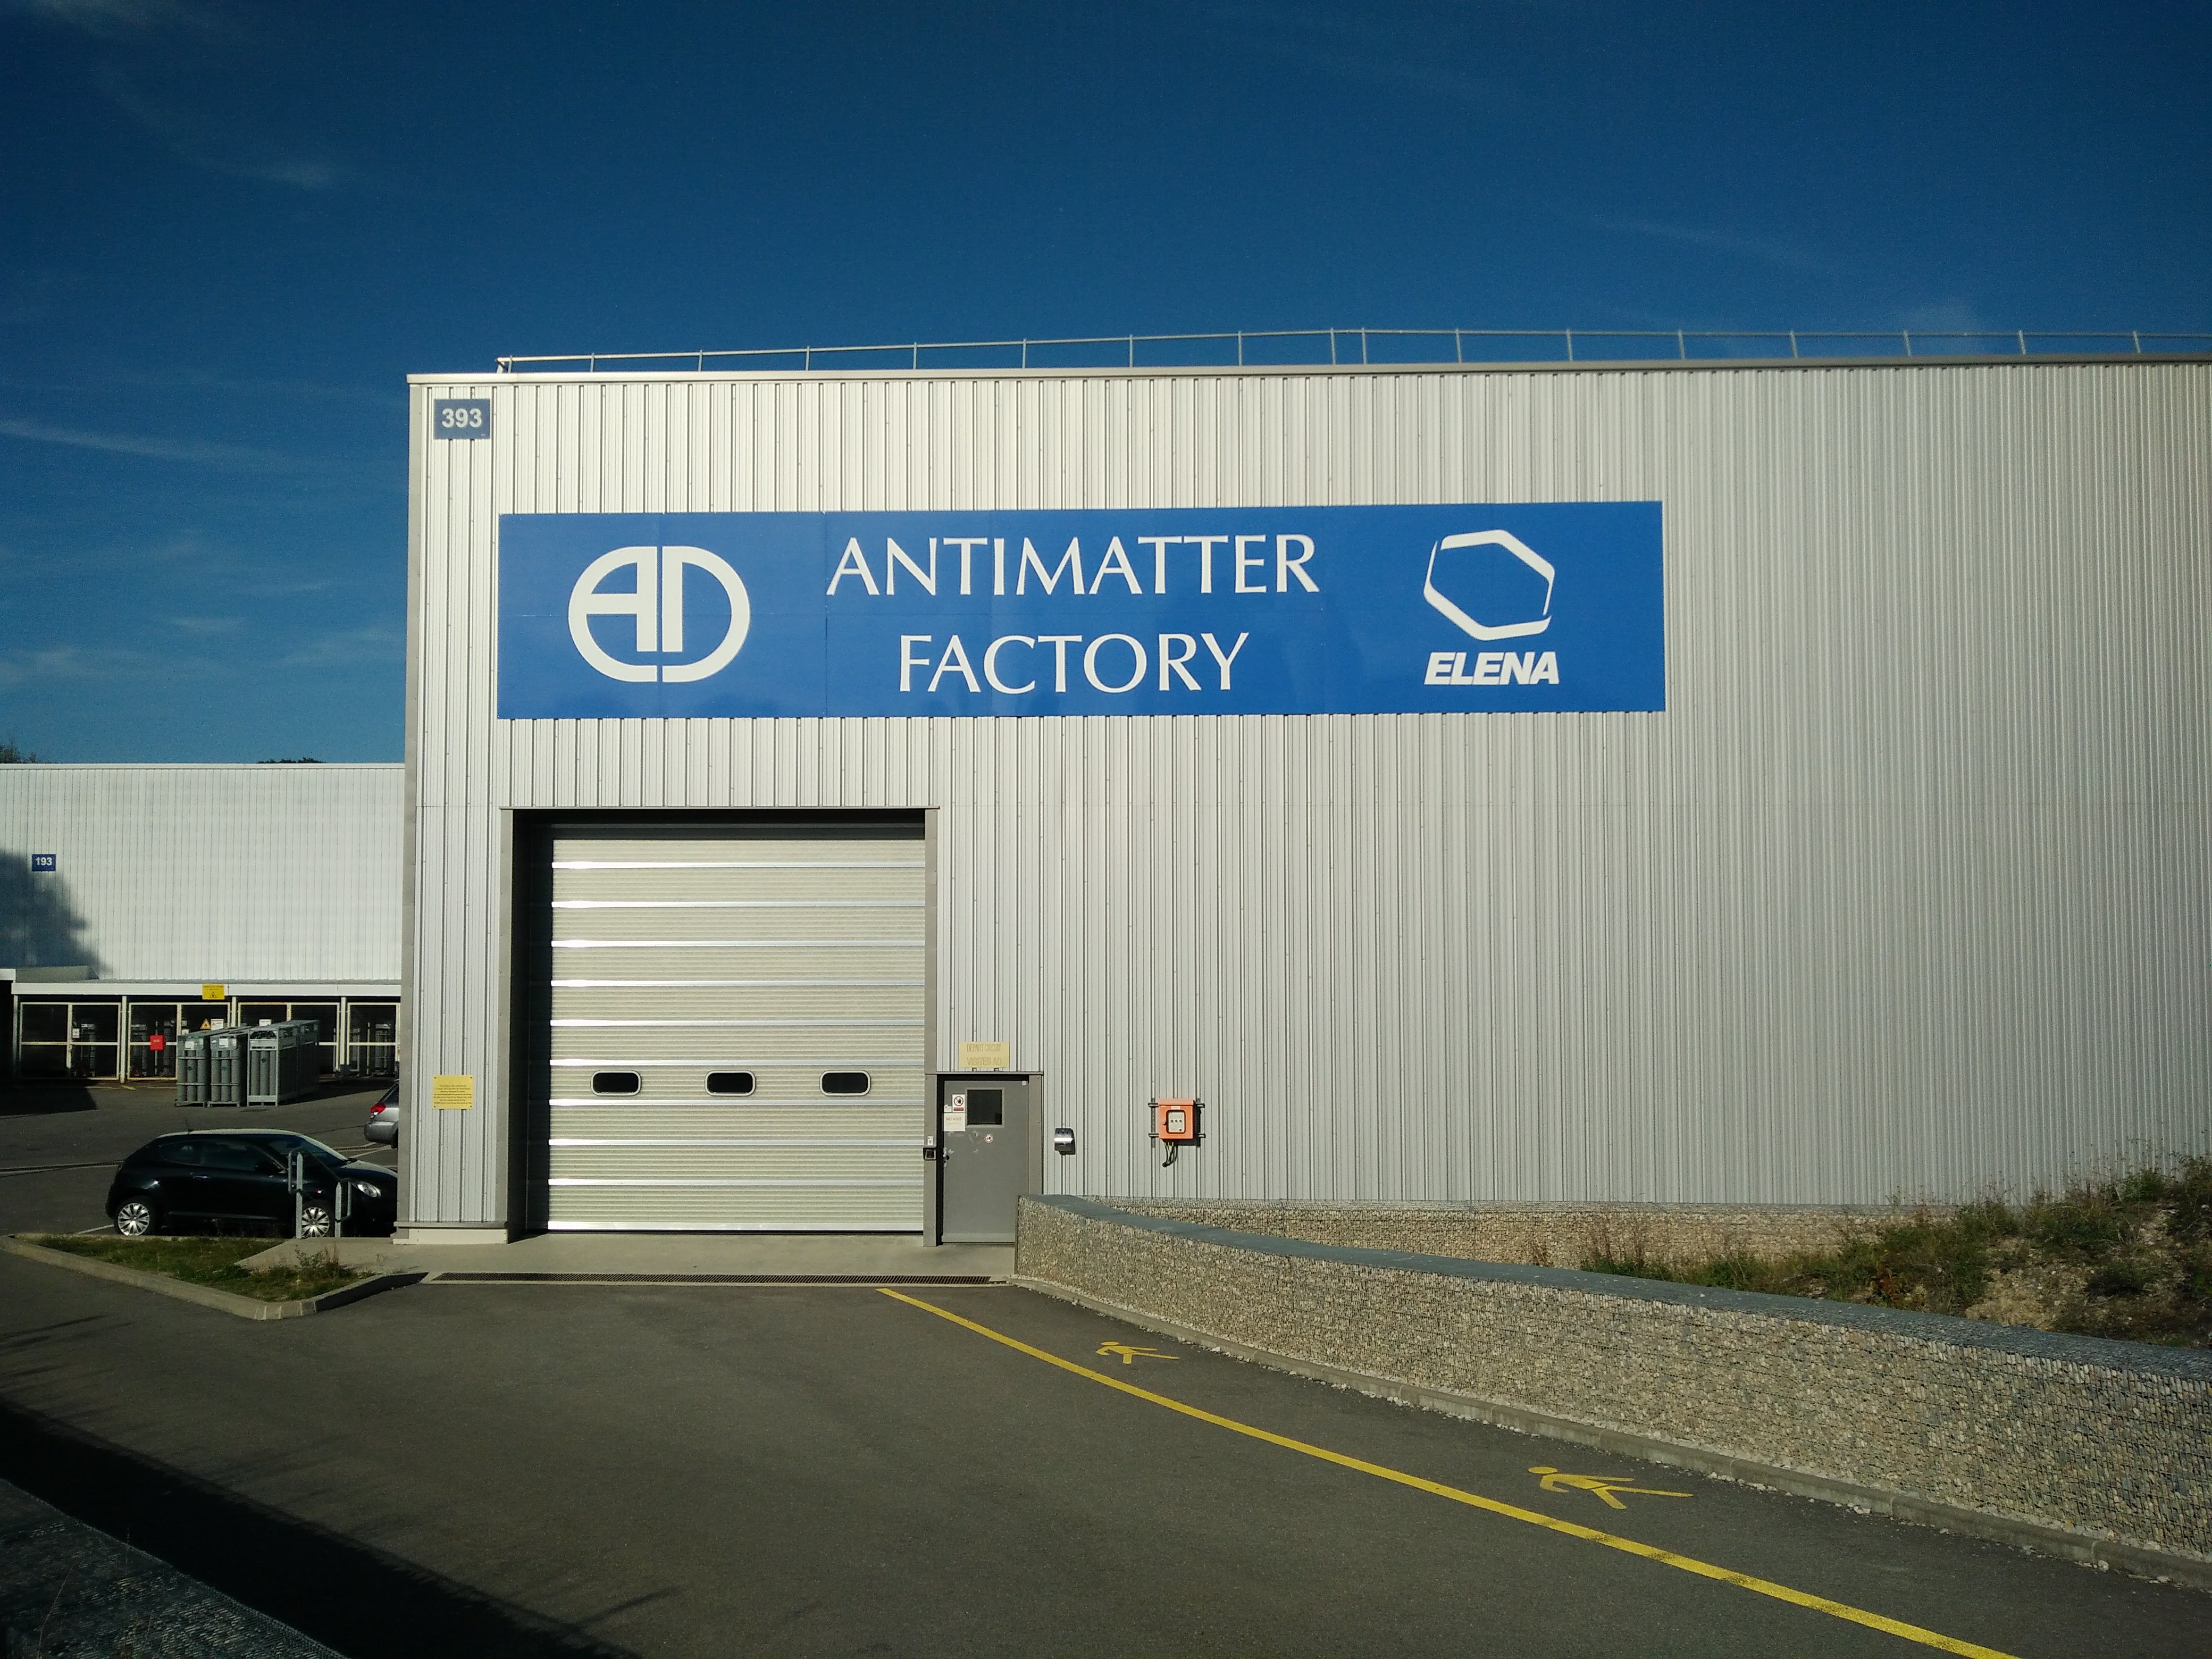
\includegraphics[width=60mm]{antimatter_factory}
\hspace{10mm}
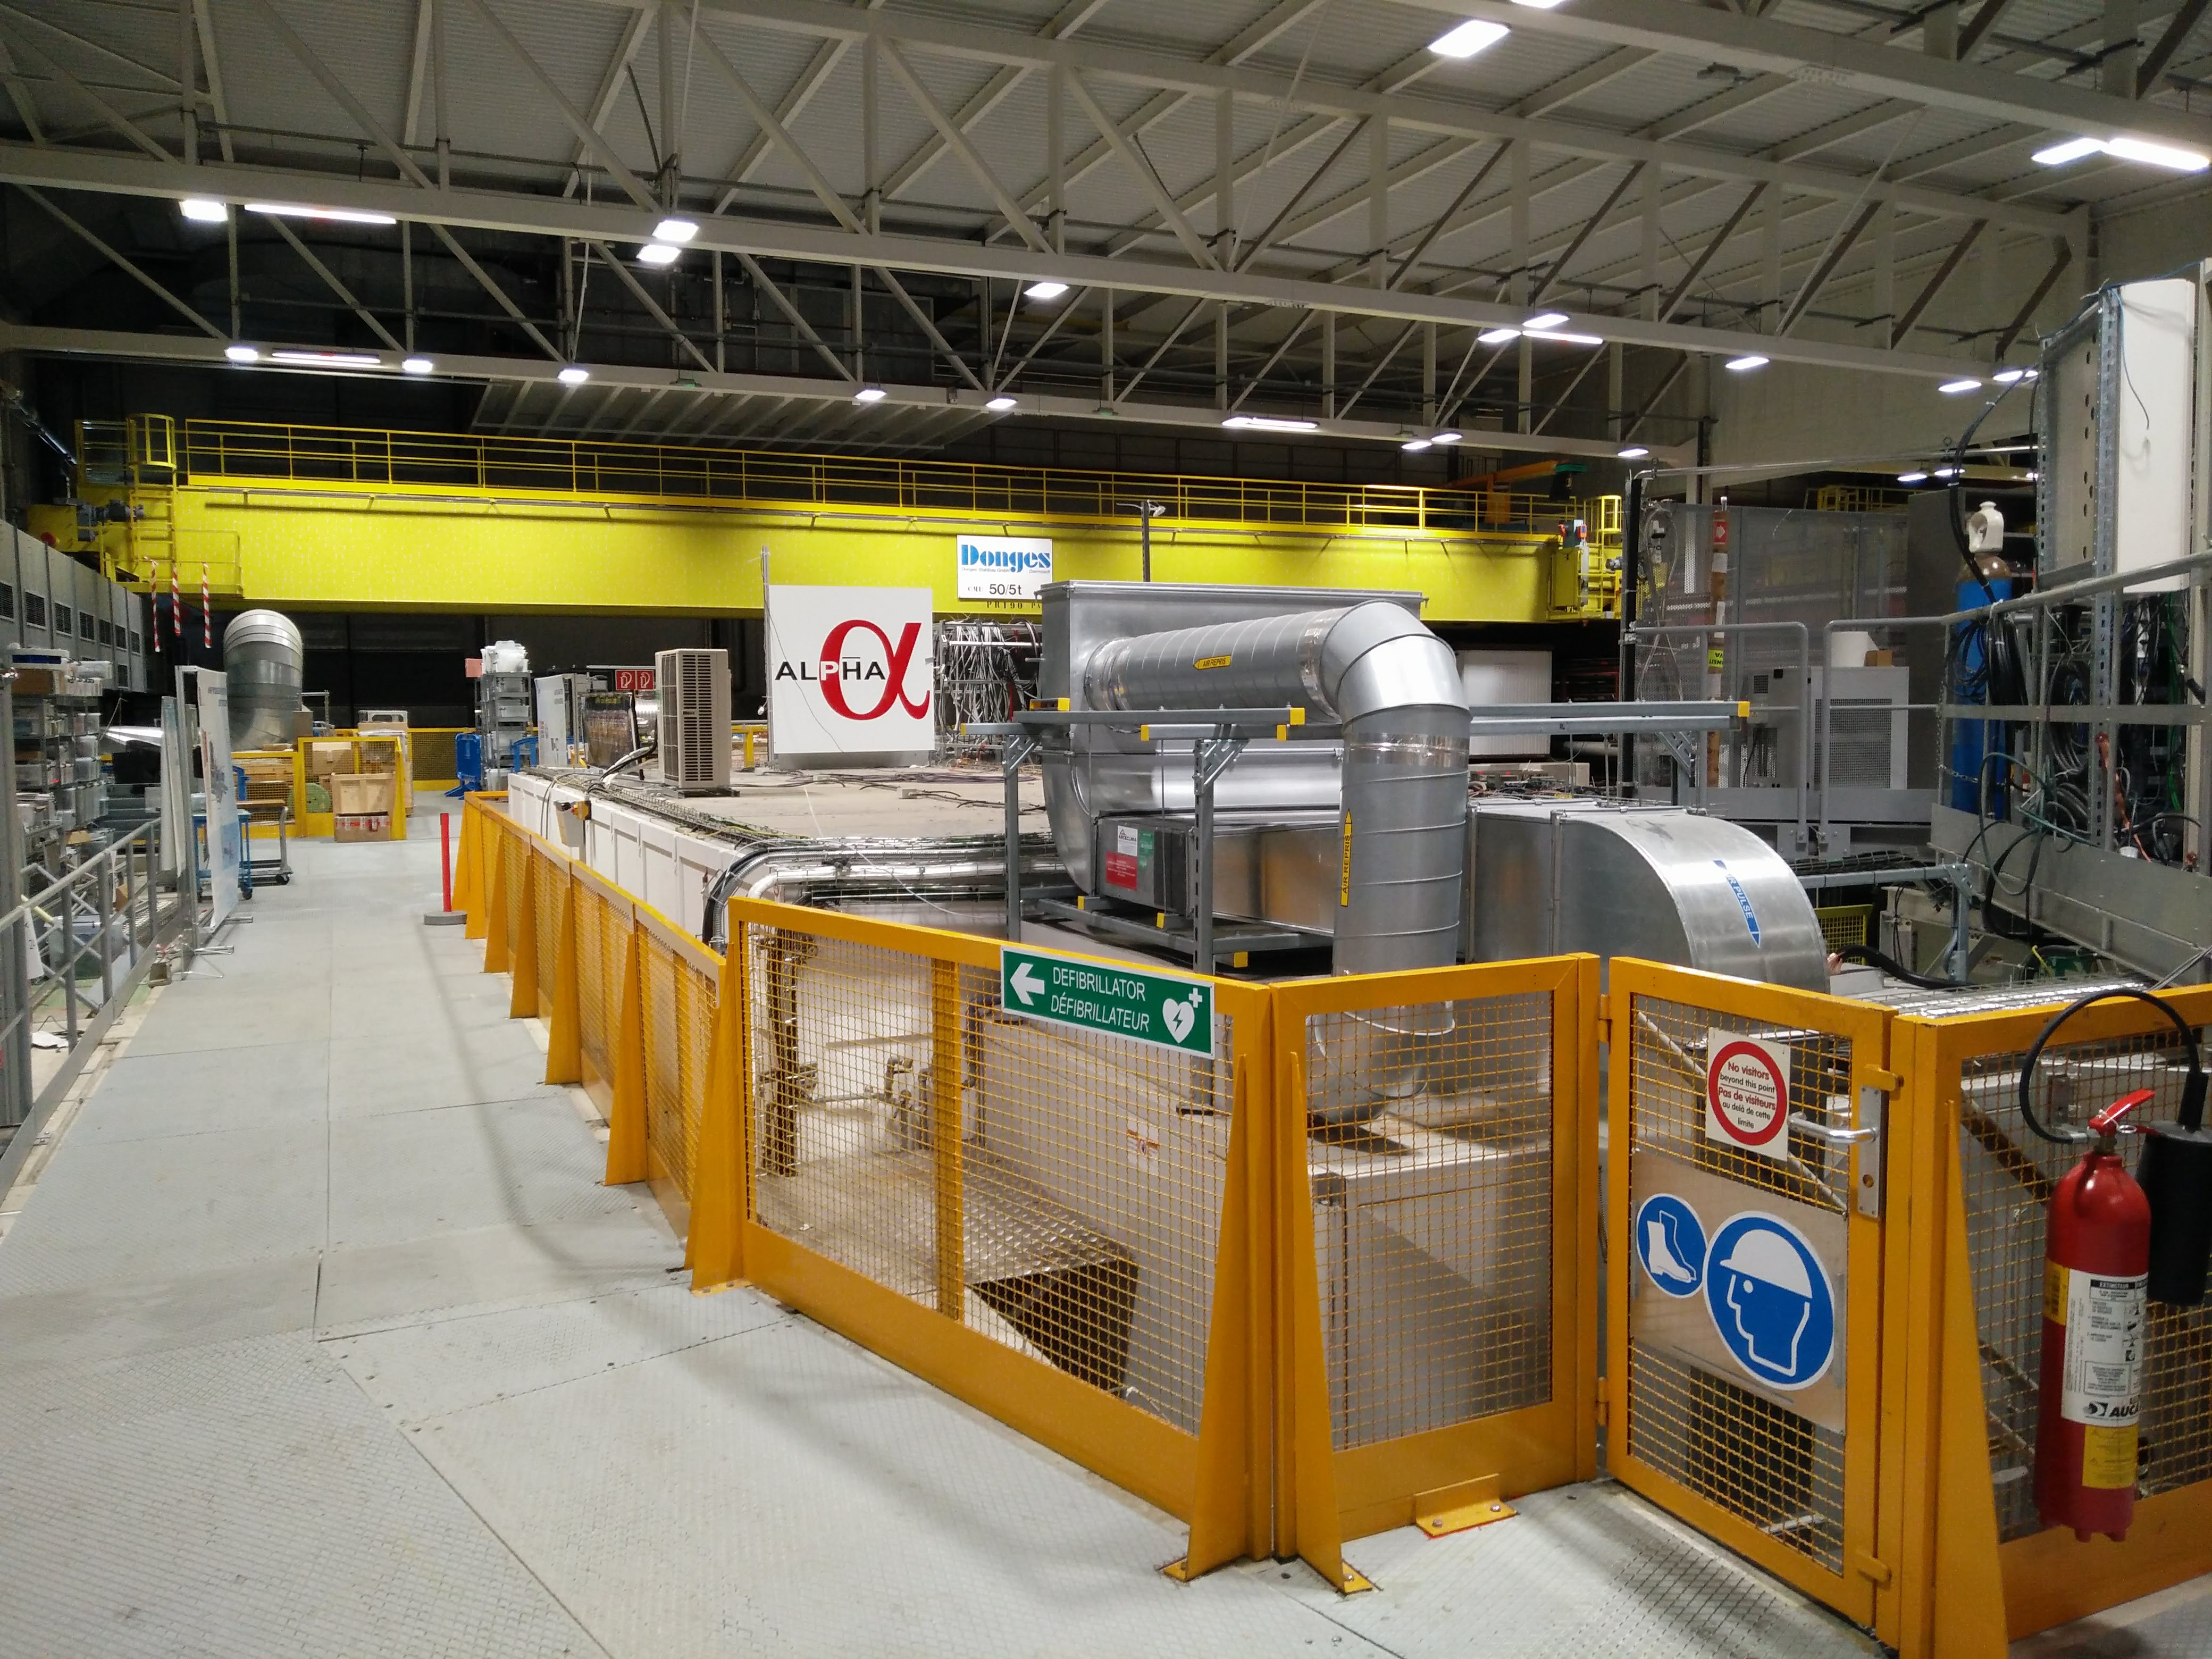
\includegraphics[width=60mm]{alpha_hall}

\caption{Antimatter Factory (left) and ALPHA experiment hall (right)}
\end{figure}

ALPHA has some important components that make the research on antimatters possible. These are: the Penning trap, which holds the positrons and antiprotons before we mix them to make antihydrogen, the Atom trap, which traps and holds the antihydrogen atoms, and the Annihilation vertex imaging detector, which detects the antihydrogen atoms when we allow them to annihilate and can find the point at which they annihilated. You can see the full setup of experiment in figure \ref{fig:full_map}.

\begin{figure}[h]
\centering
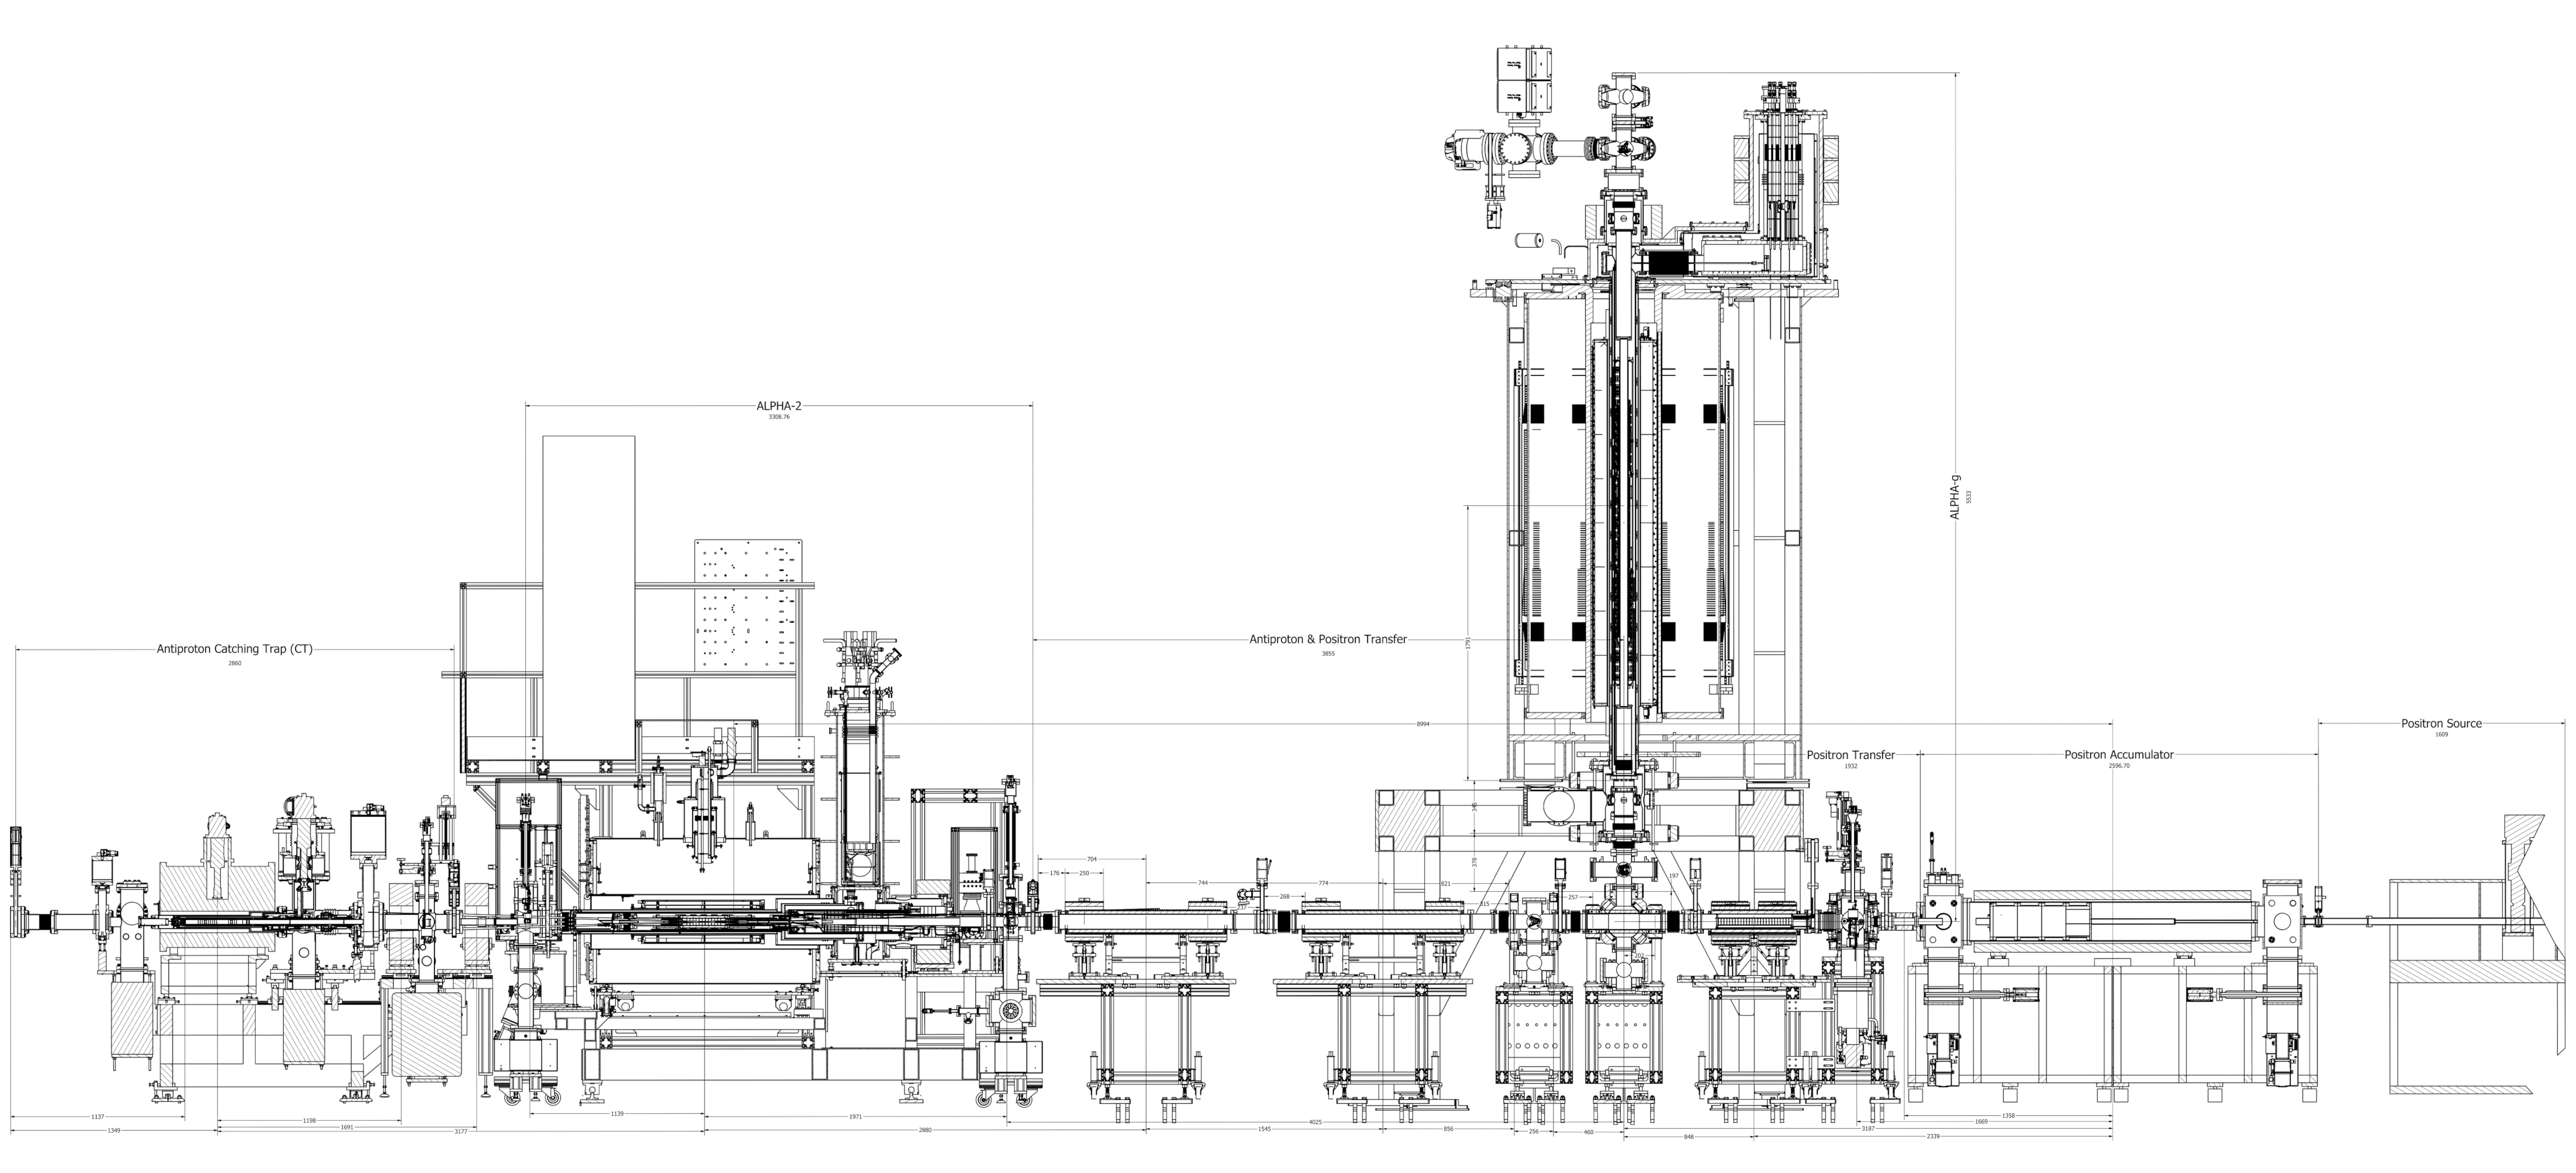
\includegraphics[scale=0.09]{full_map}
\caption{Full Setup of ALPHA experiment.}
\label{fig:full_map}
\end{figure}

Note: For pictures in these sections I have used pictures used in the web site of ALPHA.
\subsection{Magnets}
\label{Magnets} 
The ALPHA magnetic trap is a variant of a type of atom trap called an 'Ioffe trap'. This magnetic trap is used to trap antihydrogen atoms which are neutral, and electric fields can not be used to trap the particles. Such traps work because most atoms interact with a magnetic field through a property called their magnetic dipole moment. If the atom is moving in a magnetic field, it will gain and lose energy as the strength of the magnetic field near the atom changes. Making a magnetic field that increases in all directions from a central minimum point means that some atoms will gain potential energy and lose kinetic energy if they move away from the minimum. Atoms that have low enough total energy will convert all of their kinetic energy to potential energy and be reflected from the higher magnetic field and be trapped. You can think of this like a marble rolling in a bowl -- a slow-moving marble can't reach the edge of the bowl and will be `trapped' in the bowl.


\begin{figure}[h]
\centering
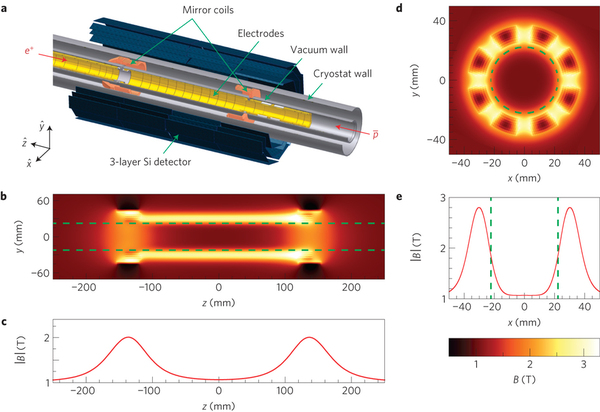
\includegraphics[scale=0.4]{magnets-trap}
\hspace{15mm}
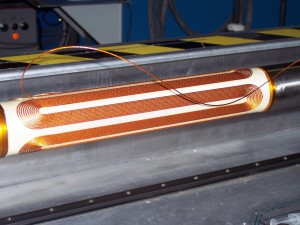
\includegraphics[scale=0.52]{magnet}
\caption{ALPHA Magnetic Trap}
\end{figure}


\subsection{Detectors}
The ALPHA neutral trap is surrounded by a complex particle detector, called the Silicon Vertex Detector (SVD). The SVD could be described as a four-megapixel 3D camera, it 'sees' inside the ALPHA -apparatus and is sensitive enough to tell us where and when a single annihilation event occurs. In ALPHA, the antihydrogen atoms annihilate mainly at the gold-coated trap walls, but occasionally the annihilation can take place in the vacuum with the tiny amount of residual gas always present in the vacuum systems. The annihilating particles in the ALPHA trap are positron and antiproton. Positron, being a lepton, annihilates with its counterpart, electron, and produces two gamma rays. The annihilation of antiproton is a more complex event, but during the annihilation process, several energetic charged particles called pions are emitted. The pions penetrate through the ALPHA -apparatus as well as the SVD, during which a tiny amount of energy is deposited into the three thin silicon sensor layers forming the SVD. The SVD records the locations of these interactions and, using this information, constructs the pion track (helix). As there are several of these tracks, the intersection of the tracks then gives the annihilation spatial location (vertex). In addition to the annihilation events, there is also cosmic muon background the SVD records. The fingerprint of these events, however, is very different from the annihilations and they can be effectively rejected.

\begin{figure}[h]

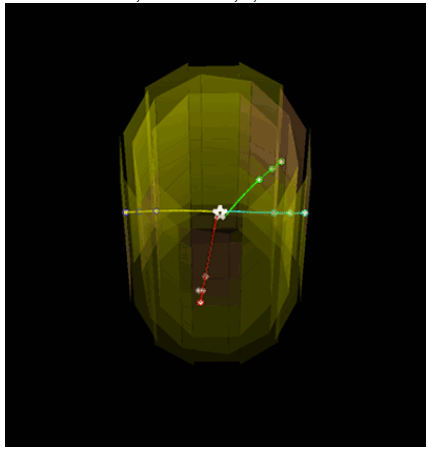
\includegraphics[scale=0.4]{detector}
\hspace{15mm}
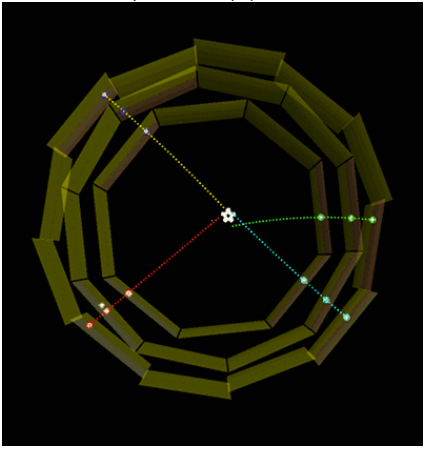
\includegraphics[scale=0.4]{detector-2}
\caption{Silicon Vertex Detector}
\end{figure}


\subsection{Penning Trap}
It is a basic and unavoidable fact in the antimatter business that to produce antihydrogen, antiprotons and positrons must be mixed. So, ALPHA must have the ability to confine and manipulate charged plasmas with reasonable efficiency and at cryogenic temperatures to boot!
This is accomplished in ALPHA through the use of Penning traps, a type of trap commonly used in plasma physics experiments to confine charged plasmas. The charge is, in fact, the difference, and indeed the dilemma faced when attempting to trap antihydrogen. Because antihydrogen is neutral, it cannot be held in a traditional Penning trap. This is where ALPHA’s unique magnetic trap comes in\footnote{\url{http://alpha.web.cern.ch/positrons}} (see \ref{Magnets}).

As for positron, antiproton and electron plasmas: a Penning trap will certainly do the trick. In a Penning trap, charged plasmas are confined in a superposition of magnetic and electric fields. You can find a great summary of fields used to trap the particles in figure \ref{trap}

\begin{figure}[h]
\centering
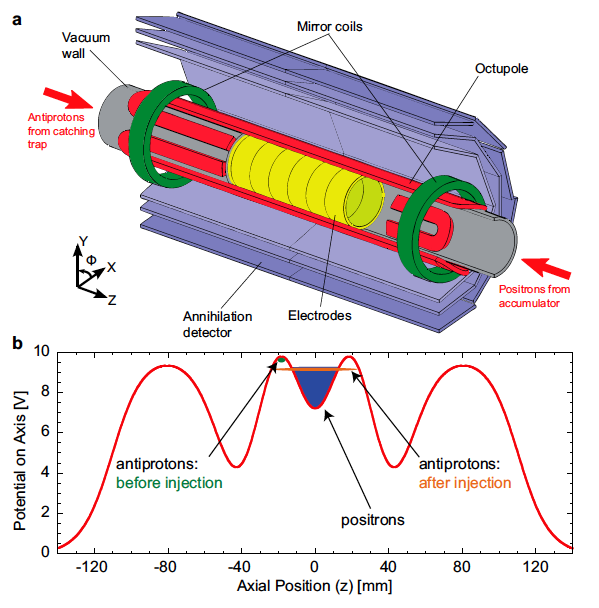
\includegraphics[scale=0.4]{penning-trap-figure}
\caption{Penning Trap}
\label{trap}
\end{figure}

\section{My Projects}

\begin{figure}[h]
\centering
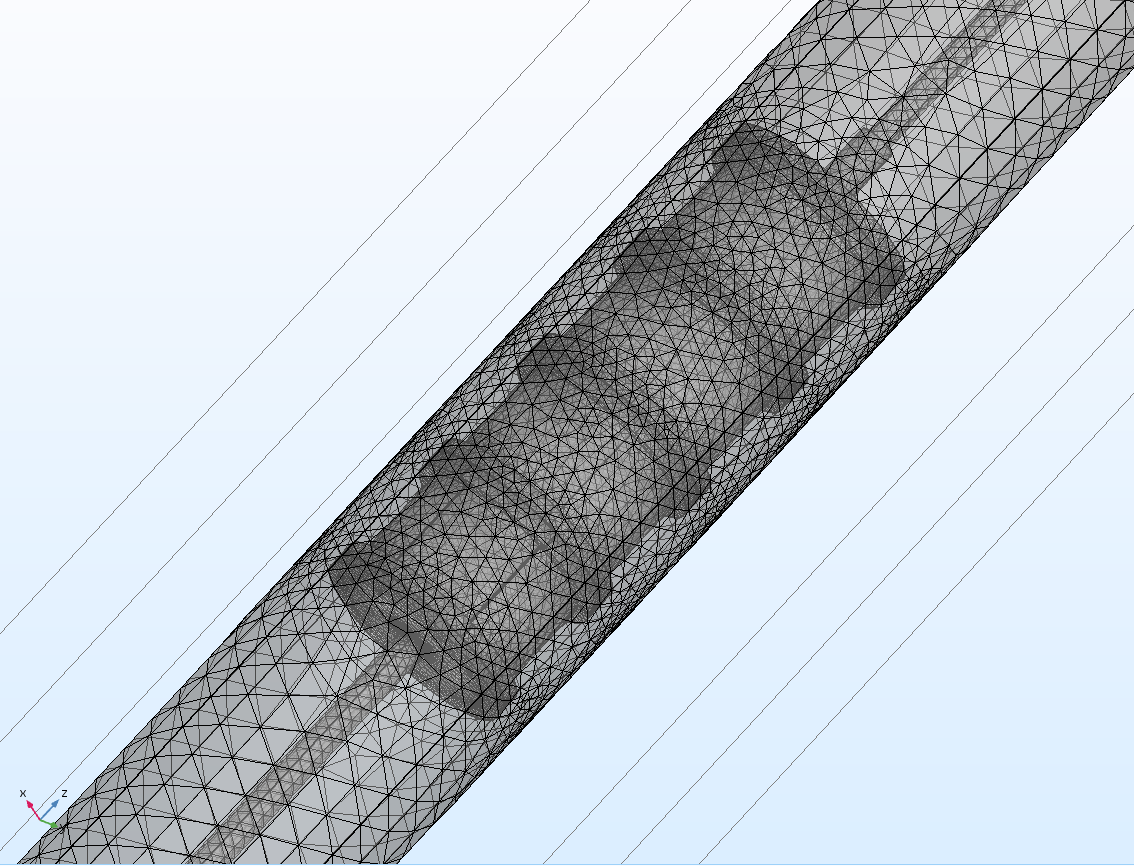
\includegraphics[scale=0.3]{Mesh}
\caption{Accumulator with fine mesh in COMSOL}
\end{figure}

\subsection{COMSOL Simulation}
When the particles are released from positron source, they are trapped in a potential well in the positron accumulator. When they are subsequently released, they travel through the magnetic beamline too the Atom Trap where they are trapped and eventually mixed with antiprotons to make antihydrogen.  positrons, on their way to reach the penning trap, expand because of the space charge. This will make the particle beam longer. So the efficiency of trapping positrons at the limited length of penning trap will decrease. because the efficient of trapping positrons is limited by the length of the penning trap. Buncher can be used to bunch the beam. The buncher used for this purpose is a set of electrodes that their potential are changed as a sinusoidal function in time.
But how do this can bunch the beam?. The answer is that when particles are released from the accumulator, the fast particles will be in the head, and the slow particles will be at the tail of the beam. So if we can tune the frequency and phase of voltage on buncher, then we can have antiresonance phenomena. so the particles that have the higher speed will feel the repulsion, and the particles with the lower speed which will arrive later to buncher will feel the attraction.  So by using this trick we will be able to bunch the particles.


In this project, First, we decided to see the expansion of the beam with simulation. So I set up a simulation with COMSOL, using "charged particles tracer" module, and after running the simulation and getting the results, we could see that the standard deviation of the Z component of the position of particles increases as they travel toward penning trap. because the real beamline was very long (11meters), and the limitation of computational resources, I set the simulation in three steps: Short beamline, Long beamline, Real beamline. in all of the simulations in this section, I have connected the buncher to the ground which has zero electric potential. Because in the first step we were interested in seeing the shape of the beam without bunching them. Also, the electric potential on the electrodes of the accumulator was same as the real values used in the experiment. you can see the electric potential calculated by simulation on the central axis of the beamline cylinder in the figure \ref{potential}.

\begin{figure}[h]

\centering
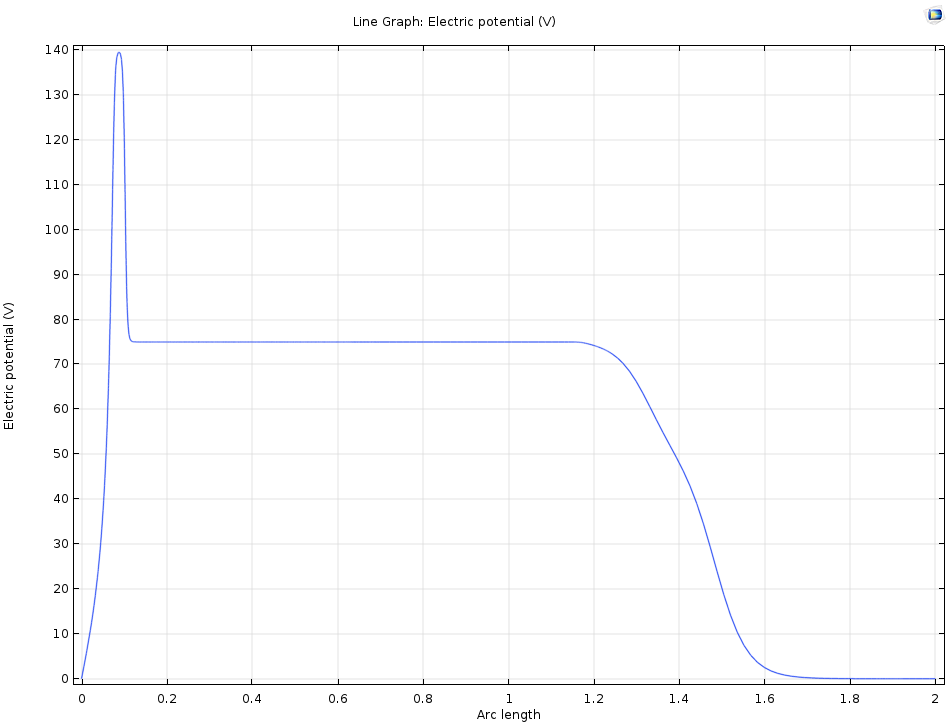
\includegraphics[width=110mm, height=30mm]{potential}
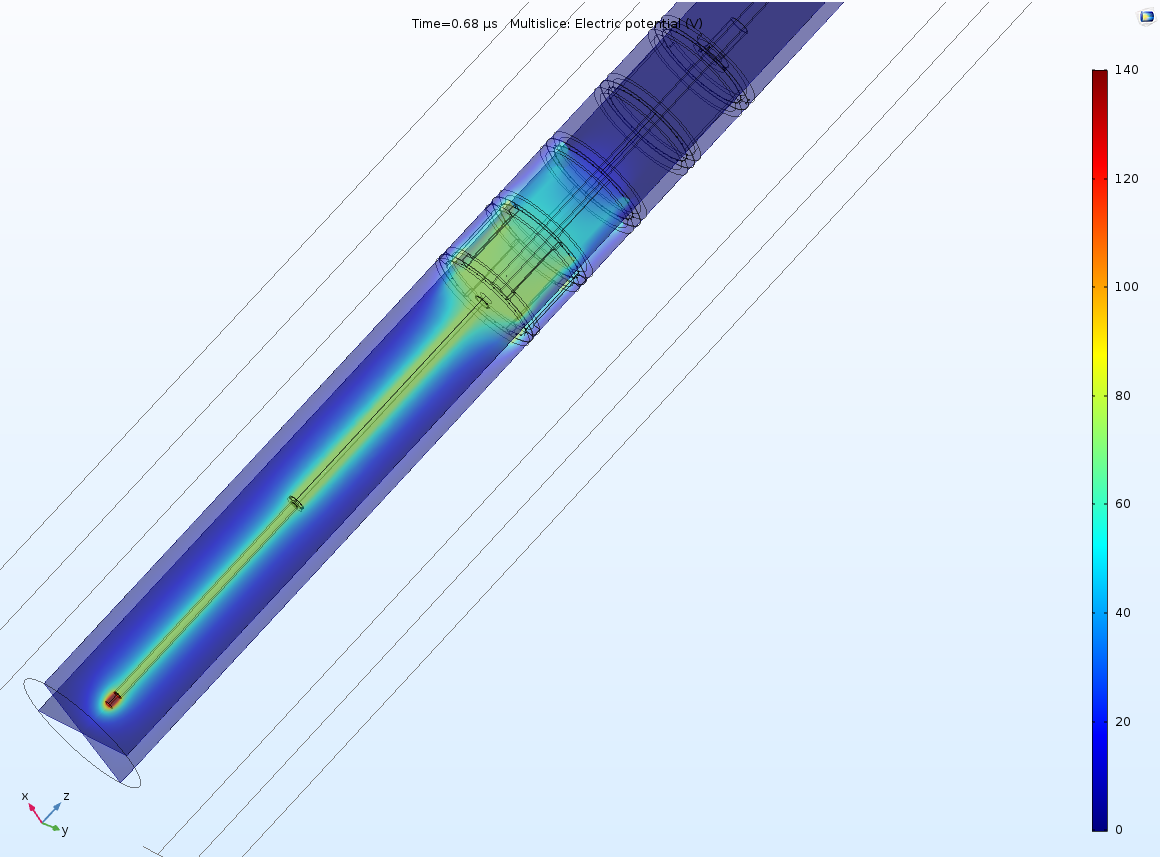
\includegraphics[width=80mm, height=40mm]{potential-3D}
\caption{Electric Potential in the Central axis of the beamline cylinder}
\label{potential}
\end{figure}

\subsubsection{Short Beamline}
In this simulation, I set the length of the beamline to be about 3 meters which only covers the accumulator and buncher. The electric potential on the electrodes of the accumulator is the same as the real values used in the experiment, but for simplicity, I have connected the buncher to the ground in order to have zero electrical potential on it. I was interested in evaluating the beam shape when they leave the buncher.

The results were quite strange. Because although we could see the expansion because of the particle-particle interaction and space charge, the results were showing a strange decrease in the standard deviation of the z position of the particles. and the depth of the well in the std plot was getting significant as the number of particles was increasing. You can find these results in figure \ref{short}. Because of this unexpected result, I decided to run more simulations with longer beamlines.

\begin{figure}[h!]
\centering
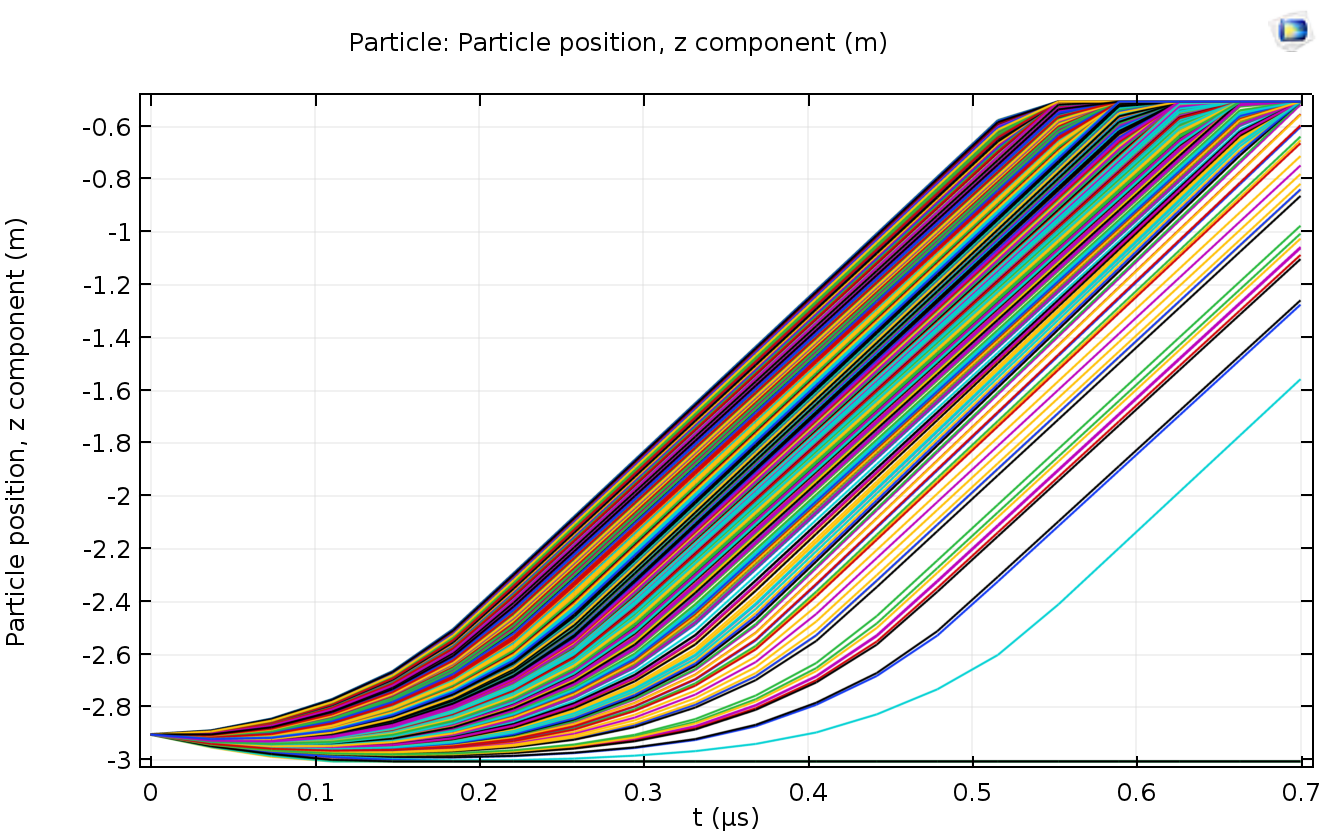
\includegraphics[width=50mm, height=50mm]{sim-in-6000}
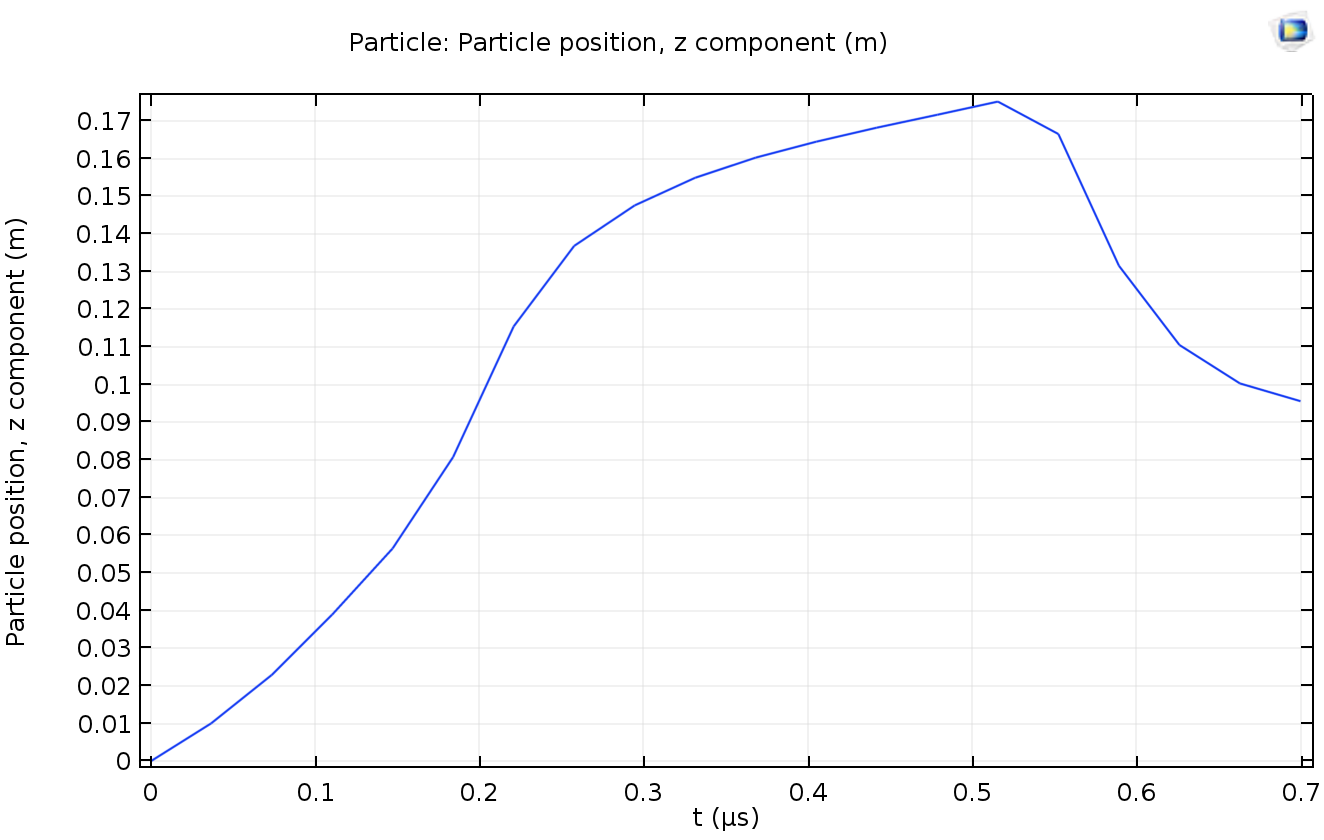
\includegraphics[width=50mm, height=50mm]{sim-std-6000}
\caption{Trajectory and Standard deviation of beam with 6000 Particles}
\label{short}
\end{figure}

\subsubsection{Long Beamline}
In this part of the simulation, I increased the length of the beamline. the size of the beamline for these simulations was about 7 meters. 

The significant result of this change was a decrease in the depth of the well at the std(z), and the more significant result was the time of simulation that increased from 18 hours to 31 hours. It was because of enlarging the simulation domain.

 finally, we noticed that the well was because of the surface that was closing the end of the beamline. Because as the particles were reaching there, they were sticking to the surface (this was because of the option that I set in preparing the simulation), so they couldn't go further away. This was resulting in a decrease in the standard deviation of the z position of particles. if this guess was true, we should see less decrease in the std on simulations with more longer beamline.
 
\begin{figure}[h]
\centering
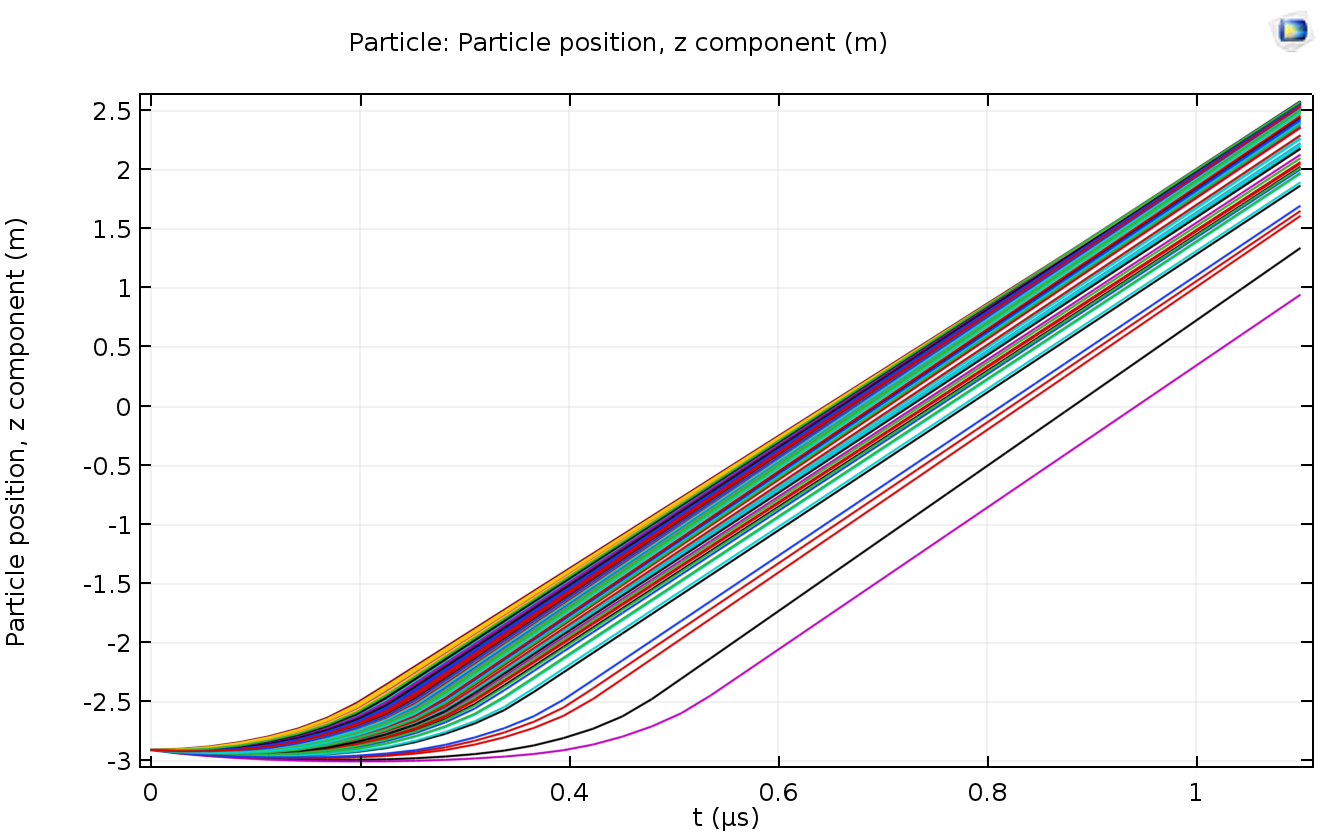
\includegraphics[width=50mm, height=50mm]{sim-in-100-long}
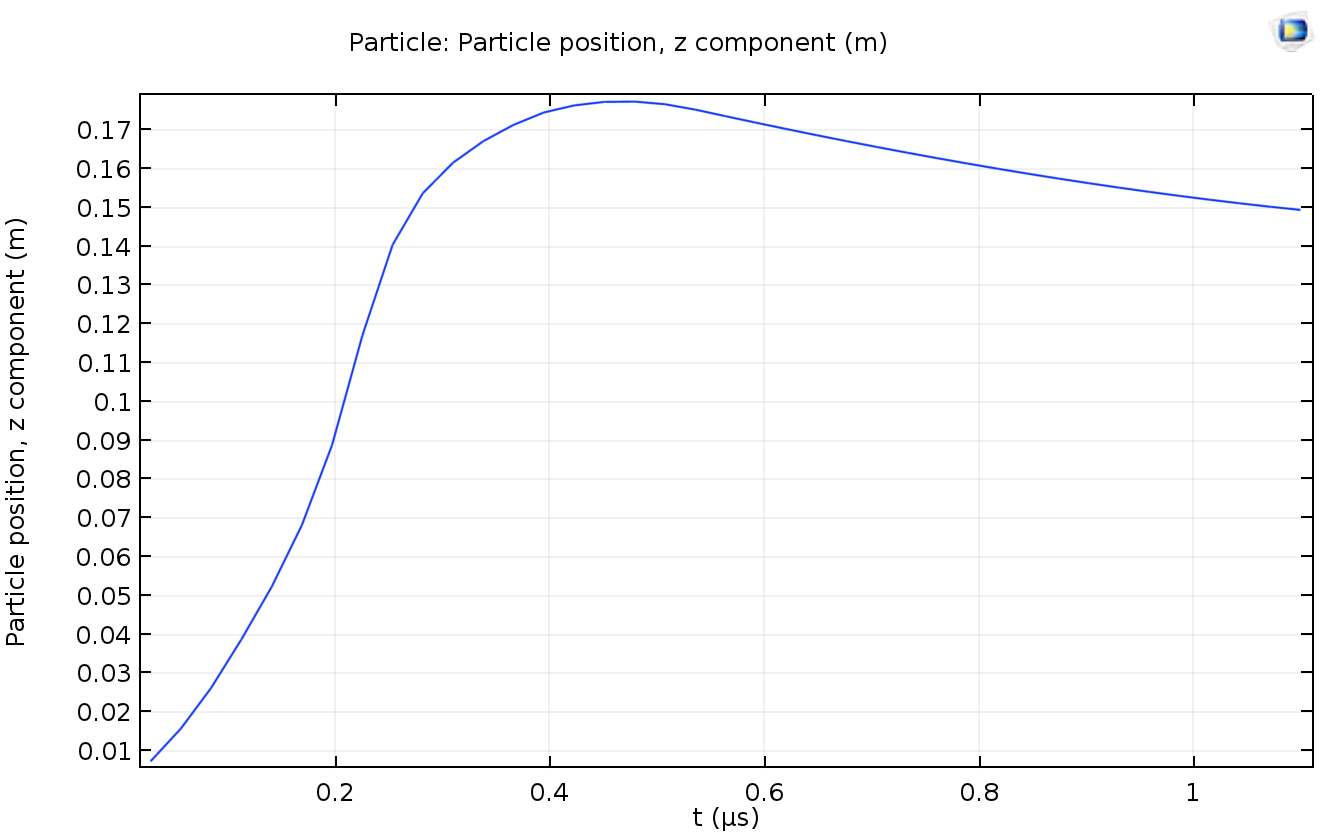
\includegraphics[width=50mm, height=50mm]{sim-std-100-long}
\caption{Trajectory and Standard deviation of beam with 6000 Particles in a beam line 6 meters long }
\end{figure}

\newpage
 
\subsubsection{Real Beamline}
this simulation was computationally costly, which took about 23 hours to simulate just five particles. The results were as we expected. There was no decrease in std(z) of particles. So this simulation was closer to the real setup than previous ones. 

\begin{figure}[h]
\centering
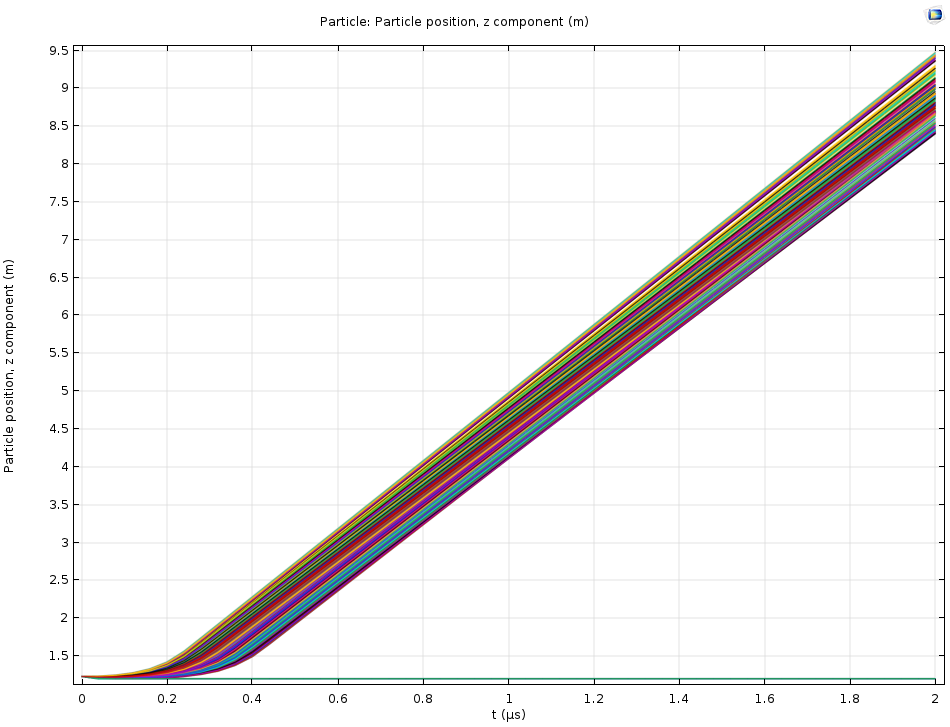
\includegraphics[width=50mm, height=50mm]{sim-in-100-11met}
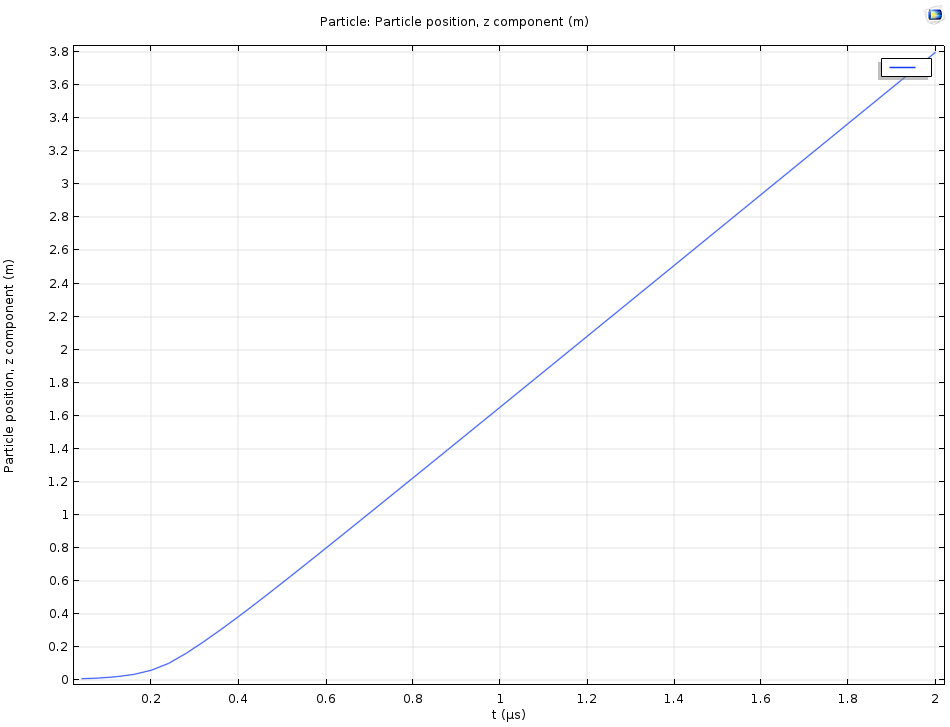
\includegraphics[width=50mm, height=50mm]{sim-std-100-11met}
\caption{Trajectory and Standard deviation of beam with 6000 Particles in a beam line 11 meters long }
\end{figure}

\subsubsection{Buncher Simulation}
As I mentioned earlier, the beam of positrons expand as they travel toward penning trap and this expansion can be suppressed using buncher. These are the results of simulation with sine potential on buncher. The sampling rate of the sine wave was 3 times the frequency of the sine function.  Although it was higher than the Nyquist frequency, we needed a higher sampling rate. I made this possible in section \ref{clus}.

\begin{figure}[h]
\centering
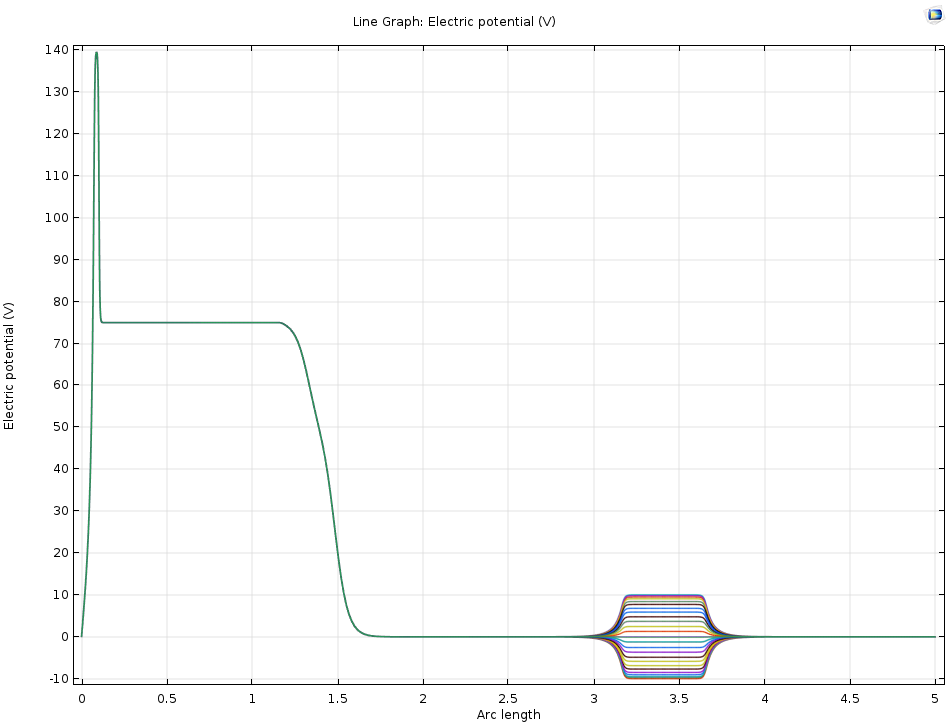
\includegraphics[width=110mm, height=40mm]{potential_buncher}
\caption{Electric Potential in the centeral axis of beam line. In this simulation buncher has $ V = 10 sin(2 \pi f t) $ potential in which $ f=10 MHz $}
\end{figure}

\begin{figure}[h]
\centering
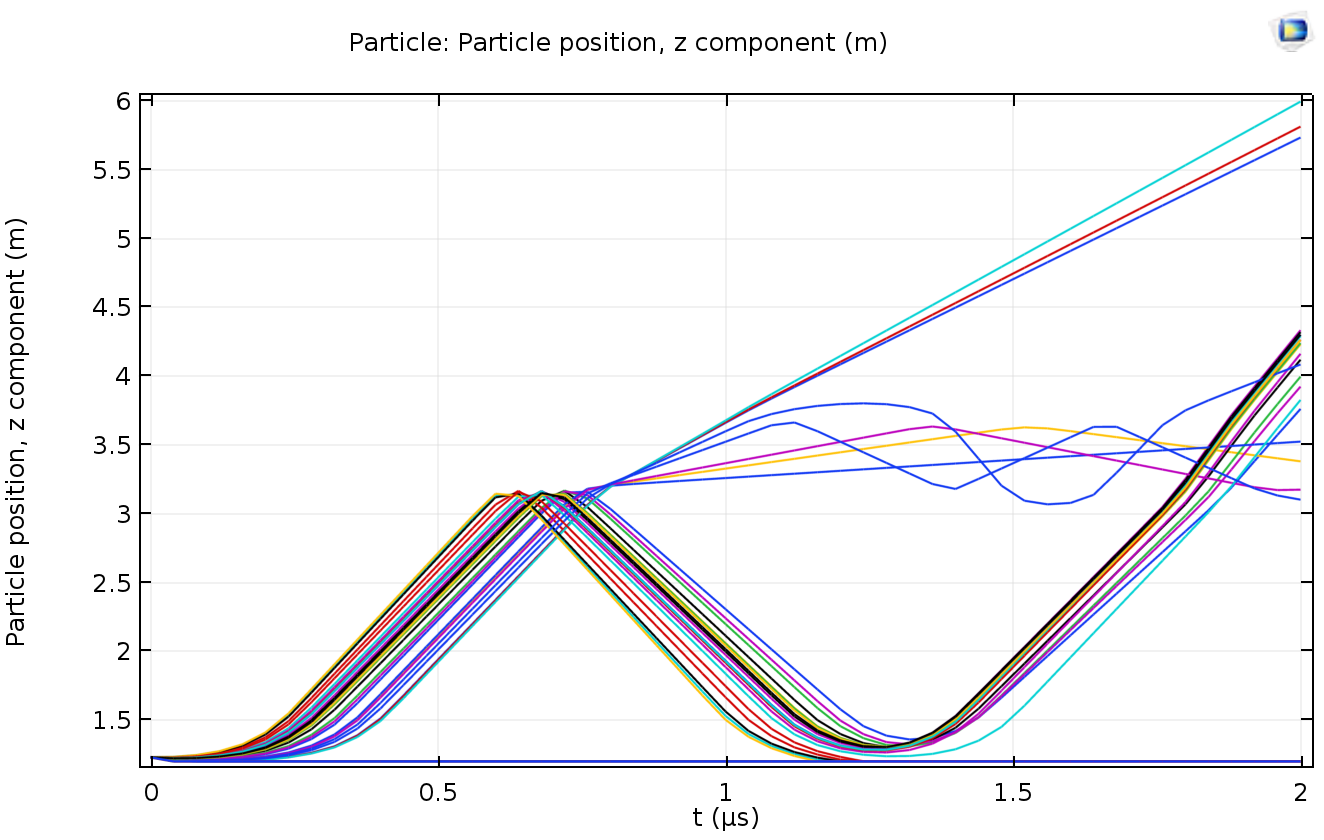
\includegraphics[width=50mm, height=50mm]{buncer-in-100V-1Mhz-50Particles}
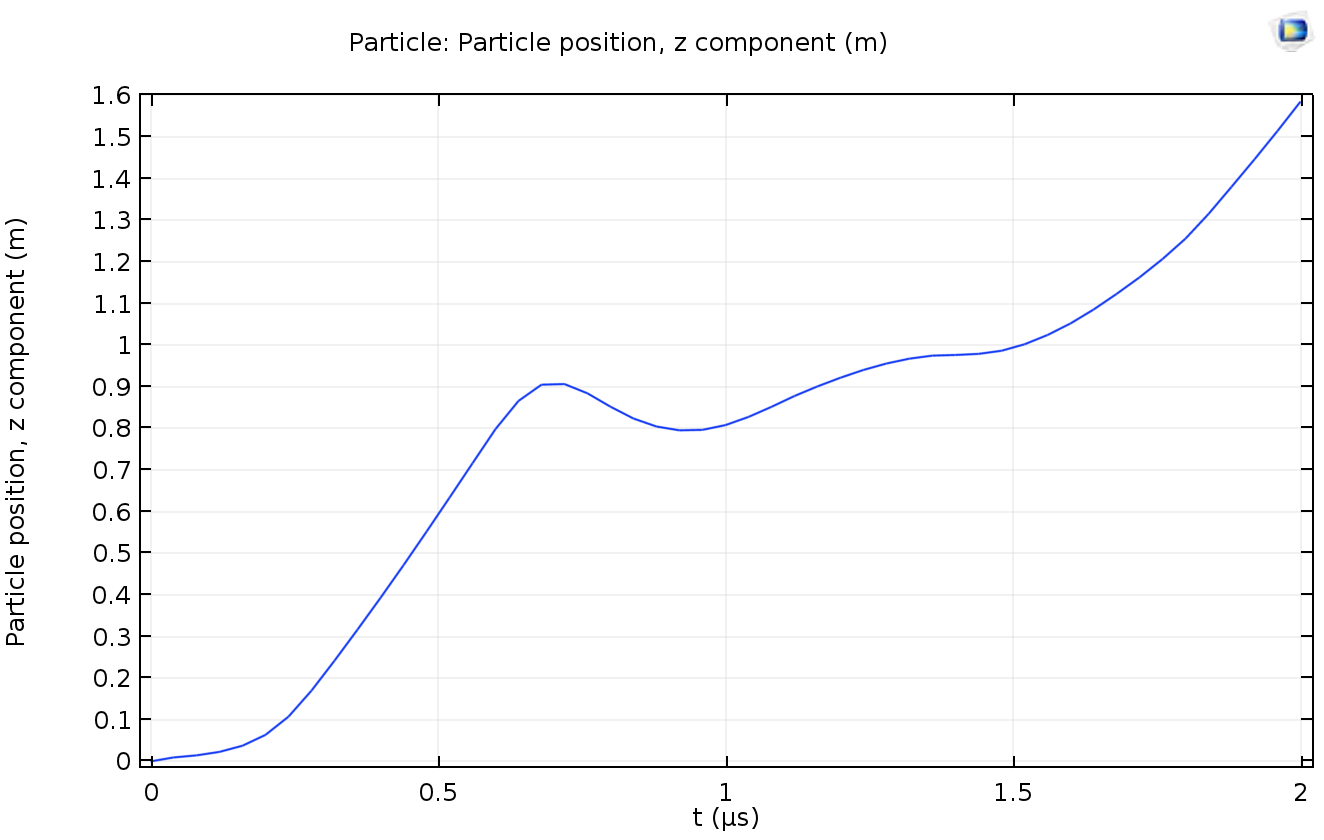
\includegraphics[width=50mm, height=50mm]{buncer-std-100V-1Mhz-50Particles}
\caption{Trajectory and Standard deviation of beam with 100 Particles in a beam line 11 meters long. In this simulation buncher has $ V = 100 sin(2 \pi f t) $ potential in which $ f=1 MHz $}
\end{figure}



\newpage


\subsection{LabVIEW Interface}

Advanced and complicated Experiments like most of the experiments at CERN are impossible to do without using advanced electronics for both collecting and analyzing data and controlling the experiment apparatus. For these advanced experiments, there are tons of parameters to be controlled, which is done in the control room (figure \ref{control}). 
So having a safe and graphical interface for this purpose has a key rule. In this project, I designed a graphical interface to control the positron accumulator source.

\begin{figure}[h]
\centering
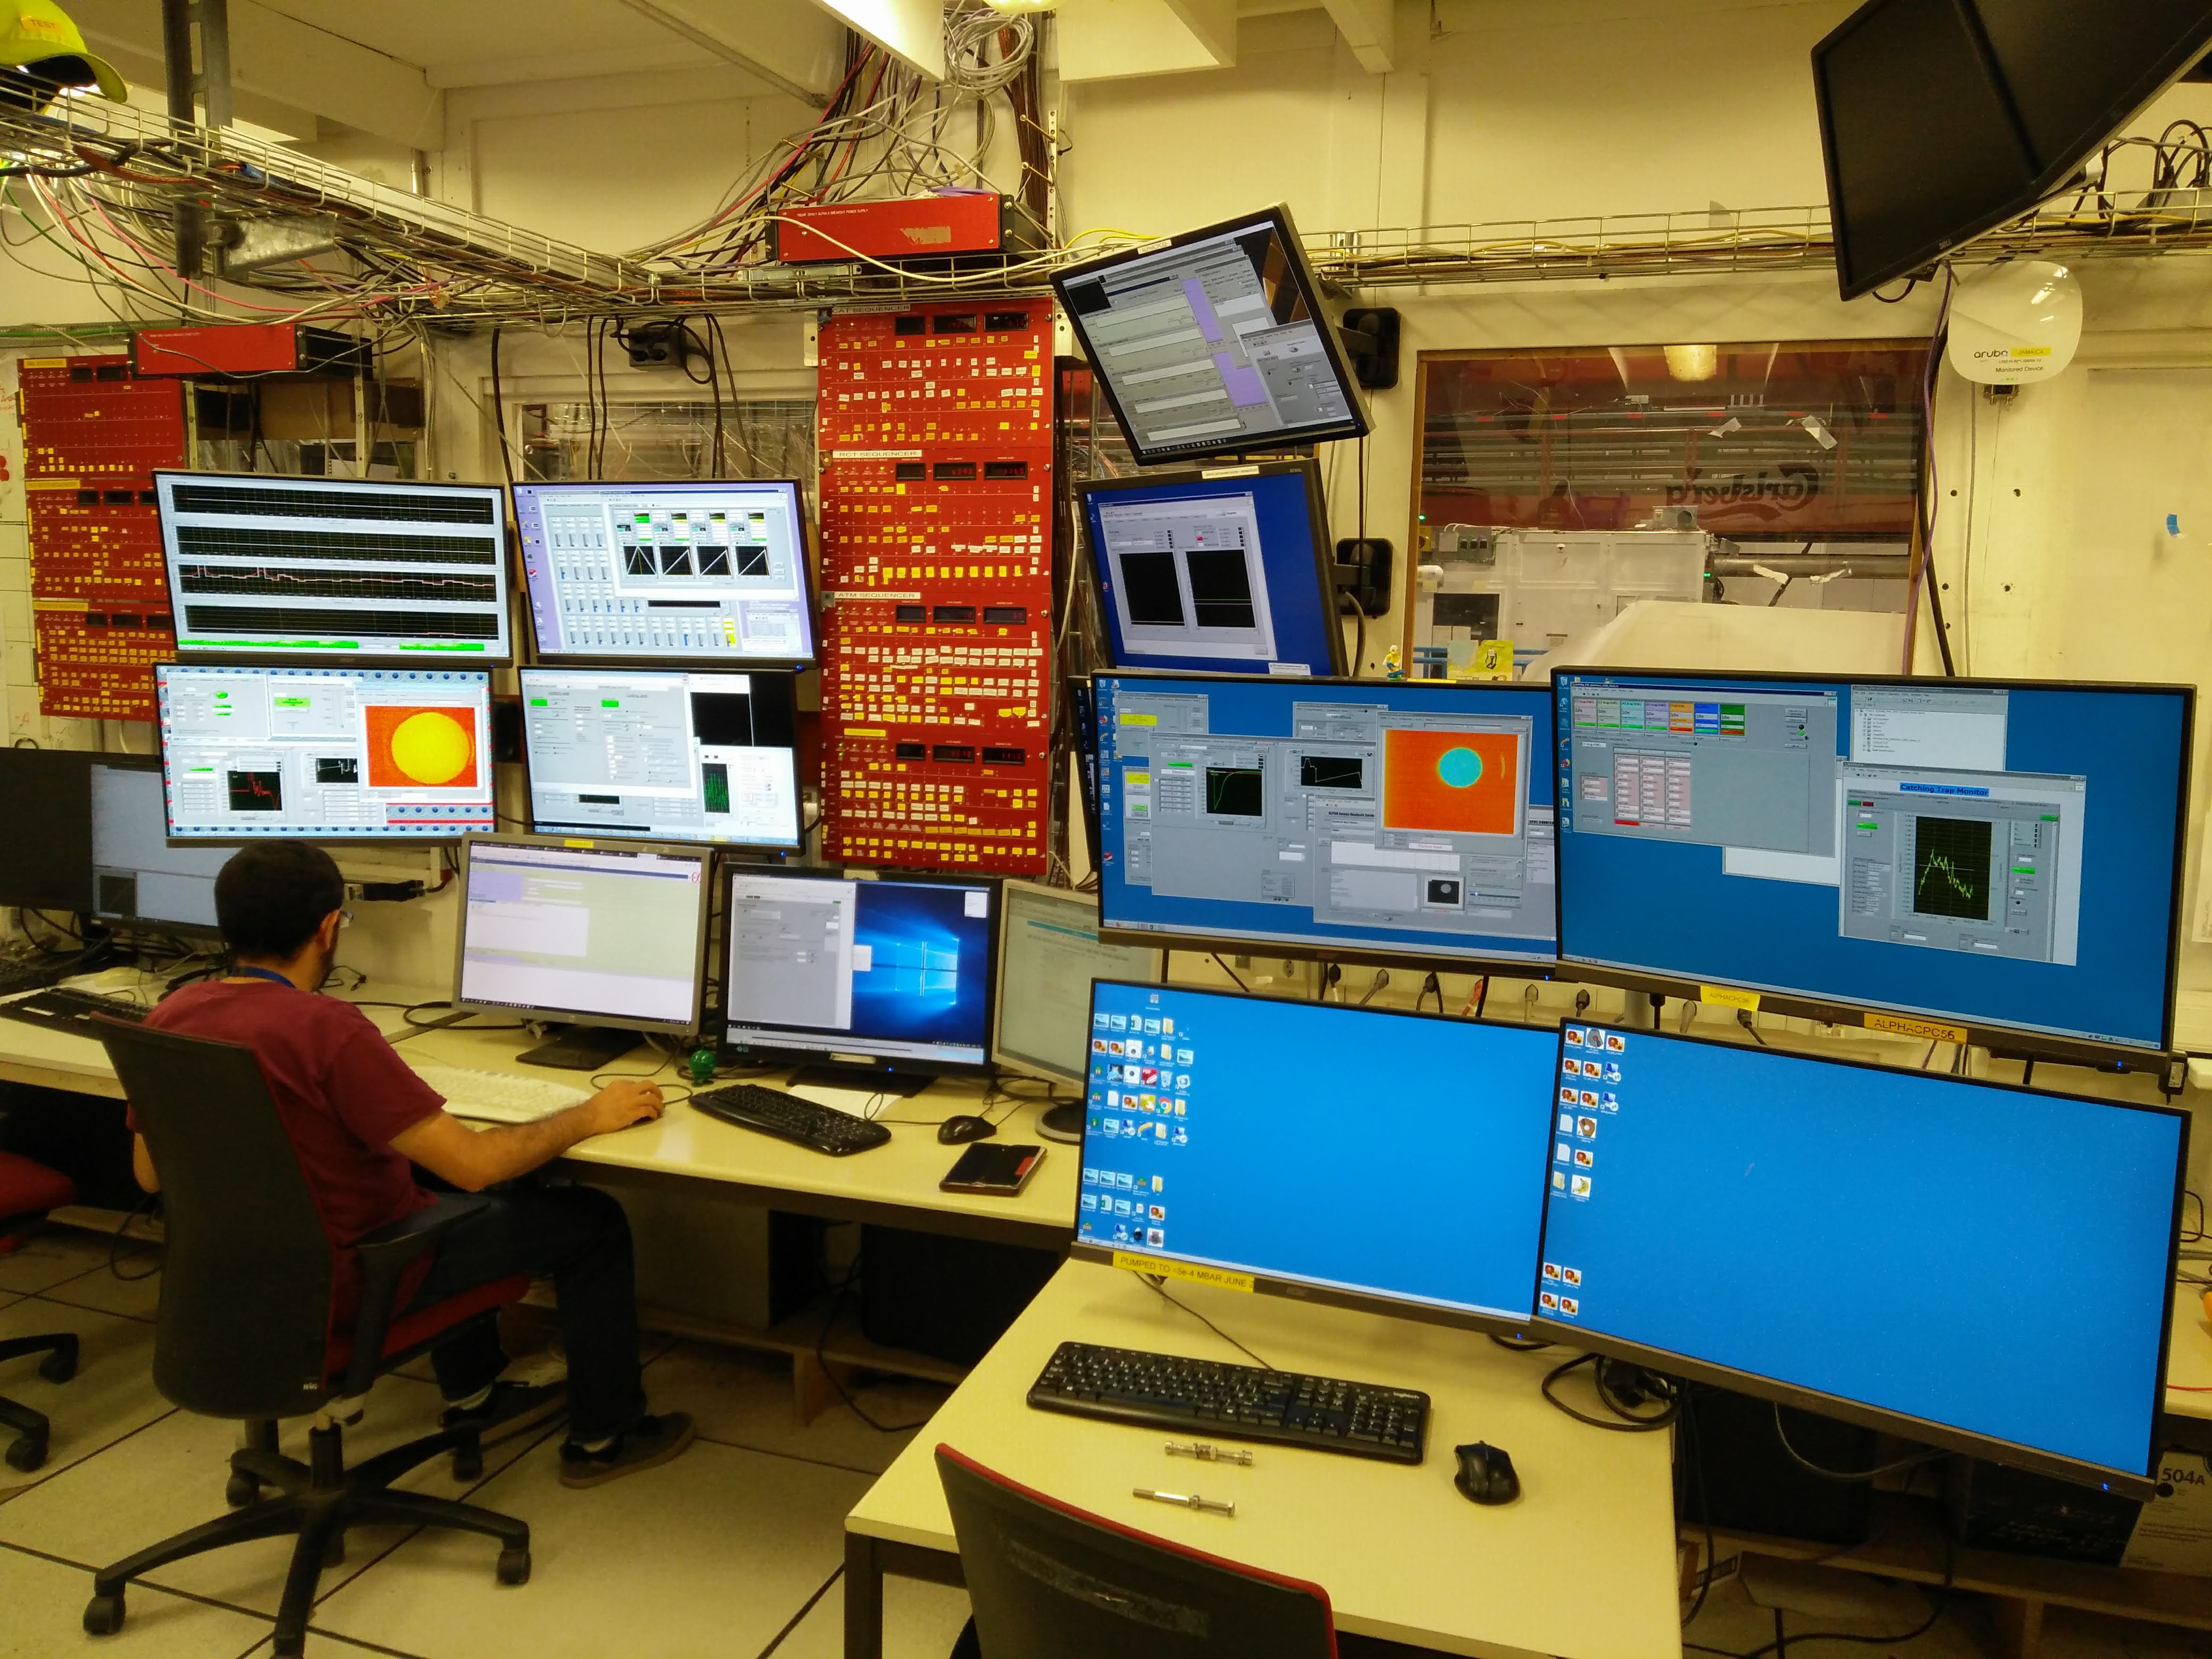
\includegraphics[width=60mm, height=60mm]{control_room}
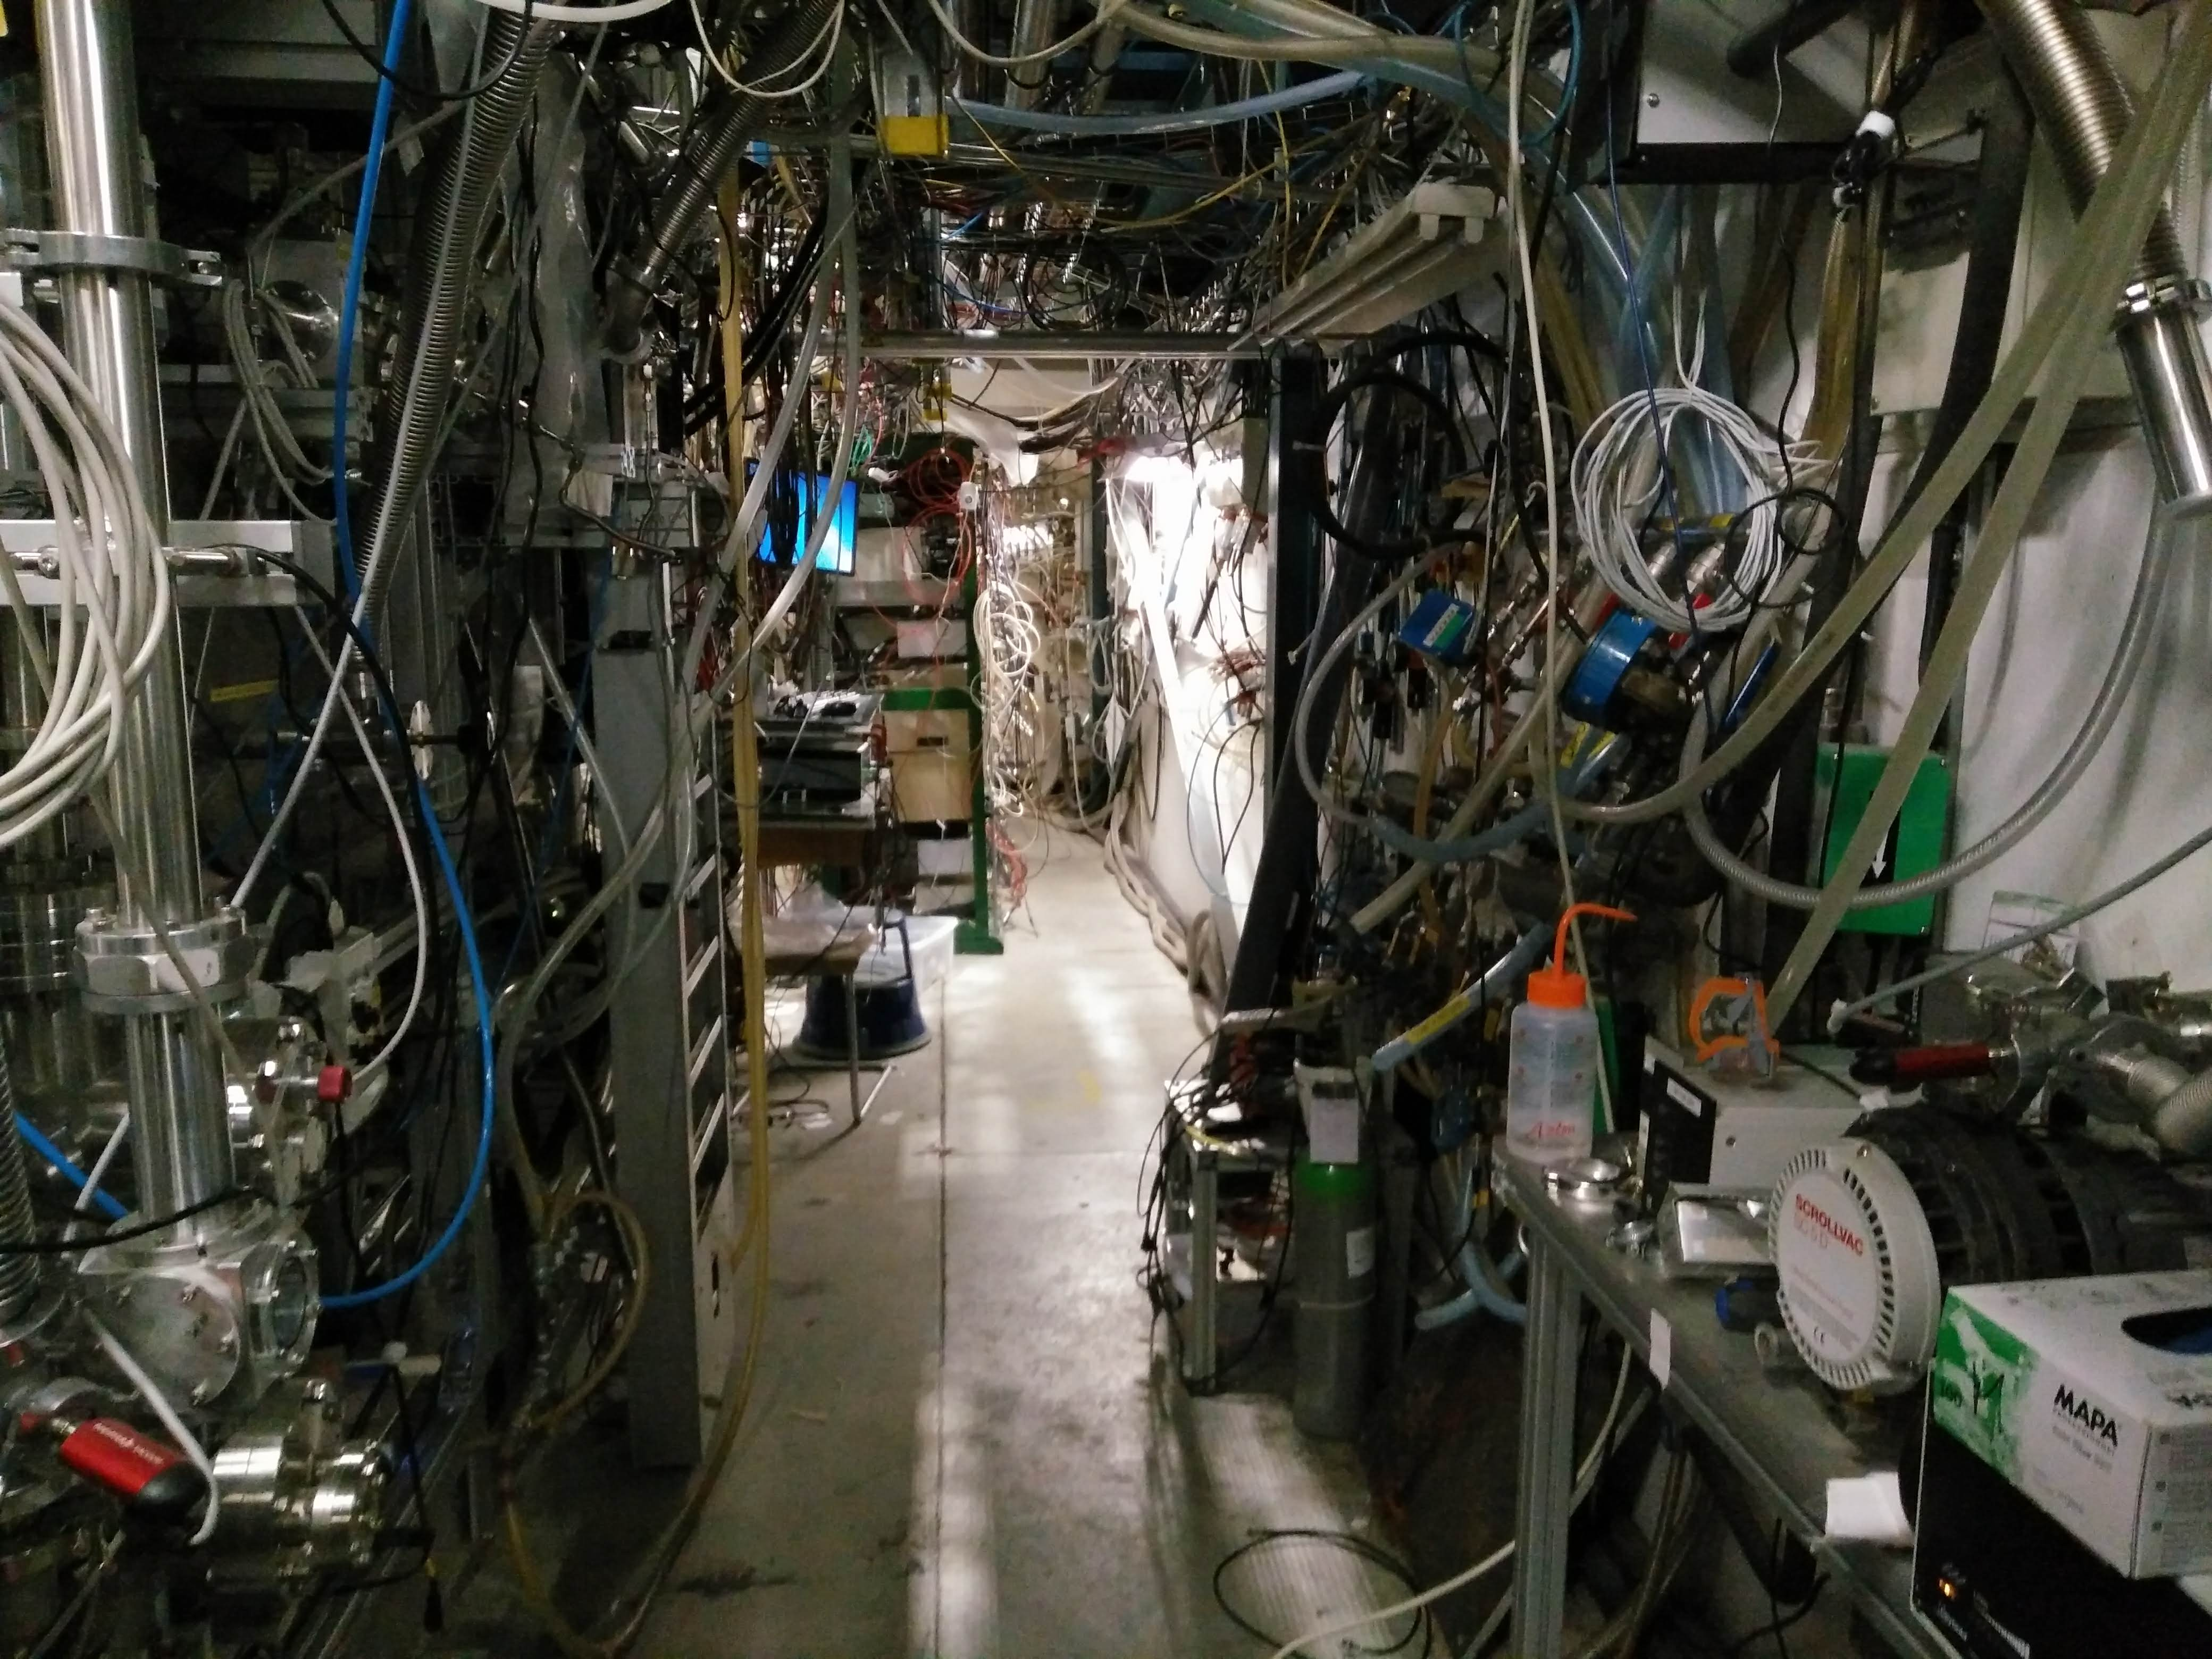
\includegraphics[width=60mm, height=60mm]{experiment_hall}
\caption{Alpha Control Room and Experiment Hall}
\label{control}
\end{figure}




\subsubsection{Positron Accumulator}

ALPHA derives its positrons from a radioactive beta-decay source containing an isotope of sodium, Na-22. This isotope, which has a conveniently long half-life of about 2.6 years, emits positrons with a large spread of kinetic energies up to about 545 keV. Such energetic positrons cannot easily be applied for antihydrogen production, so that ALPHA uses a well established technique to produce a low energy (eV) beam of positrons in vacuum.

Positrons implanted into solid material typically have a lifetime less than one nanosecond, a thousand millionth of a second. However, during that brief time most will slow down by a variety of energy loss processes to reach kinetic energies close to those characteristic of the temperature of the solid. This process is termed moderation, as the positron’s kinetic energy is lowered, or moderated. Whilst most of the positrons penetrate deep into the bulk of the material and annihilate there, about 1 percent
 stop close enough to the surface that they can diffuse back to it before they annihilate. Incredibly, most of the positrons which reach the surface are emitted into vacuum at low energy, and can be readily formed into a beam and transported, typically using magnetic guiding fields. ALPHA uses a solid film of condensed neon as its moderator; this is one of the most efficient positron moderators.
 
 
\begin{figure}[h]
\centering
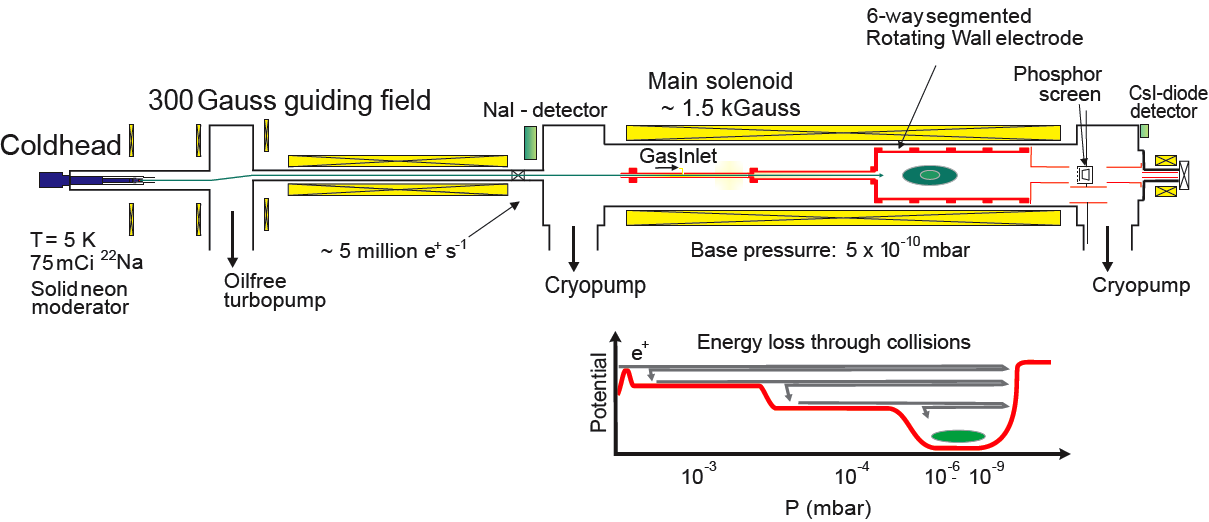
\includegraphics[width=110 mm, height=40mm]{fullsetup}
\caption{Positron Source and Accumulator}
\label{positroon}
\end{figure}

\subsubsection{Experiment Control}

The computers that control the different parameters of the experiment are located on the control platforms (figure \ref{platform}).  


\begin{figure}[h]

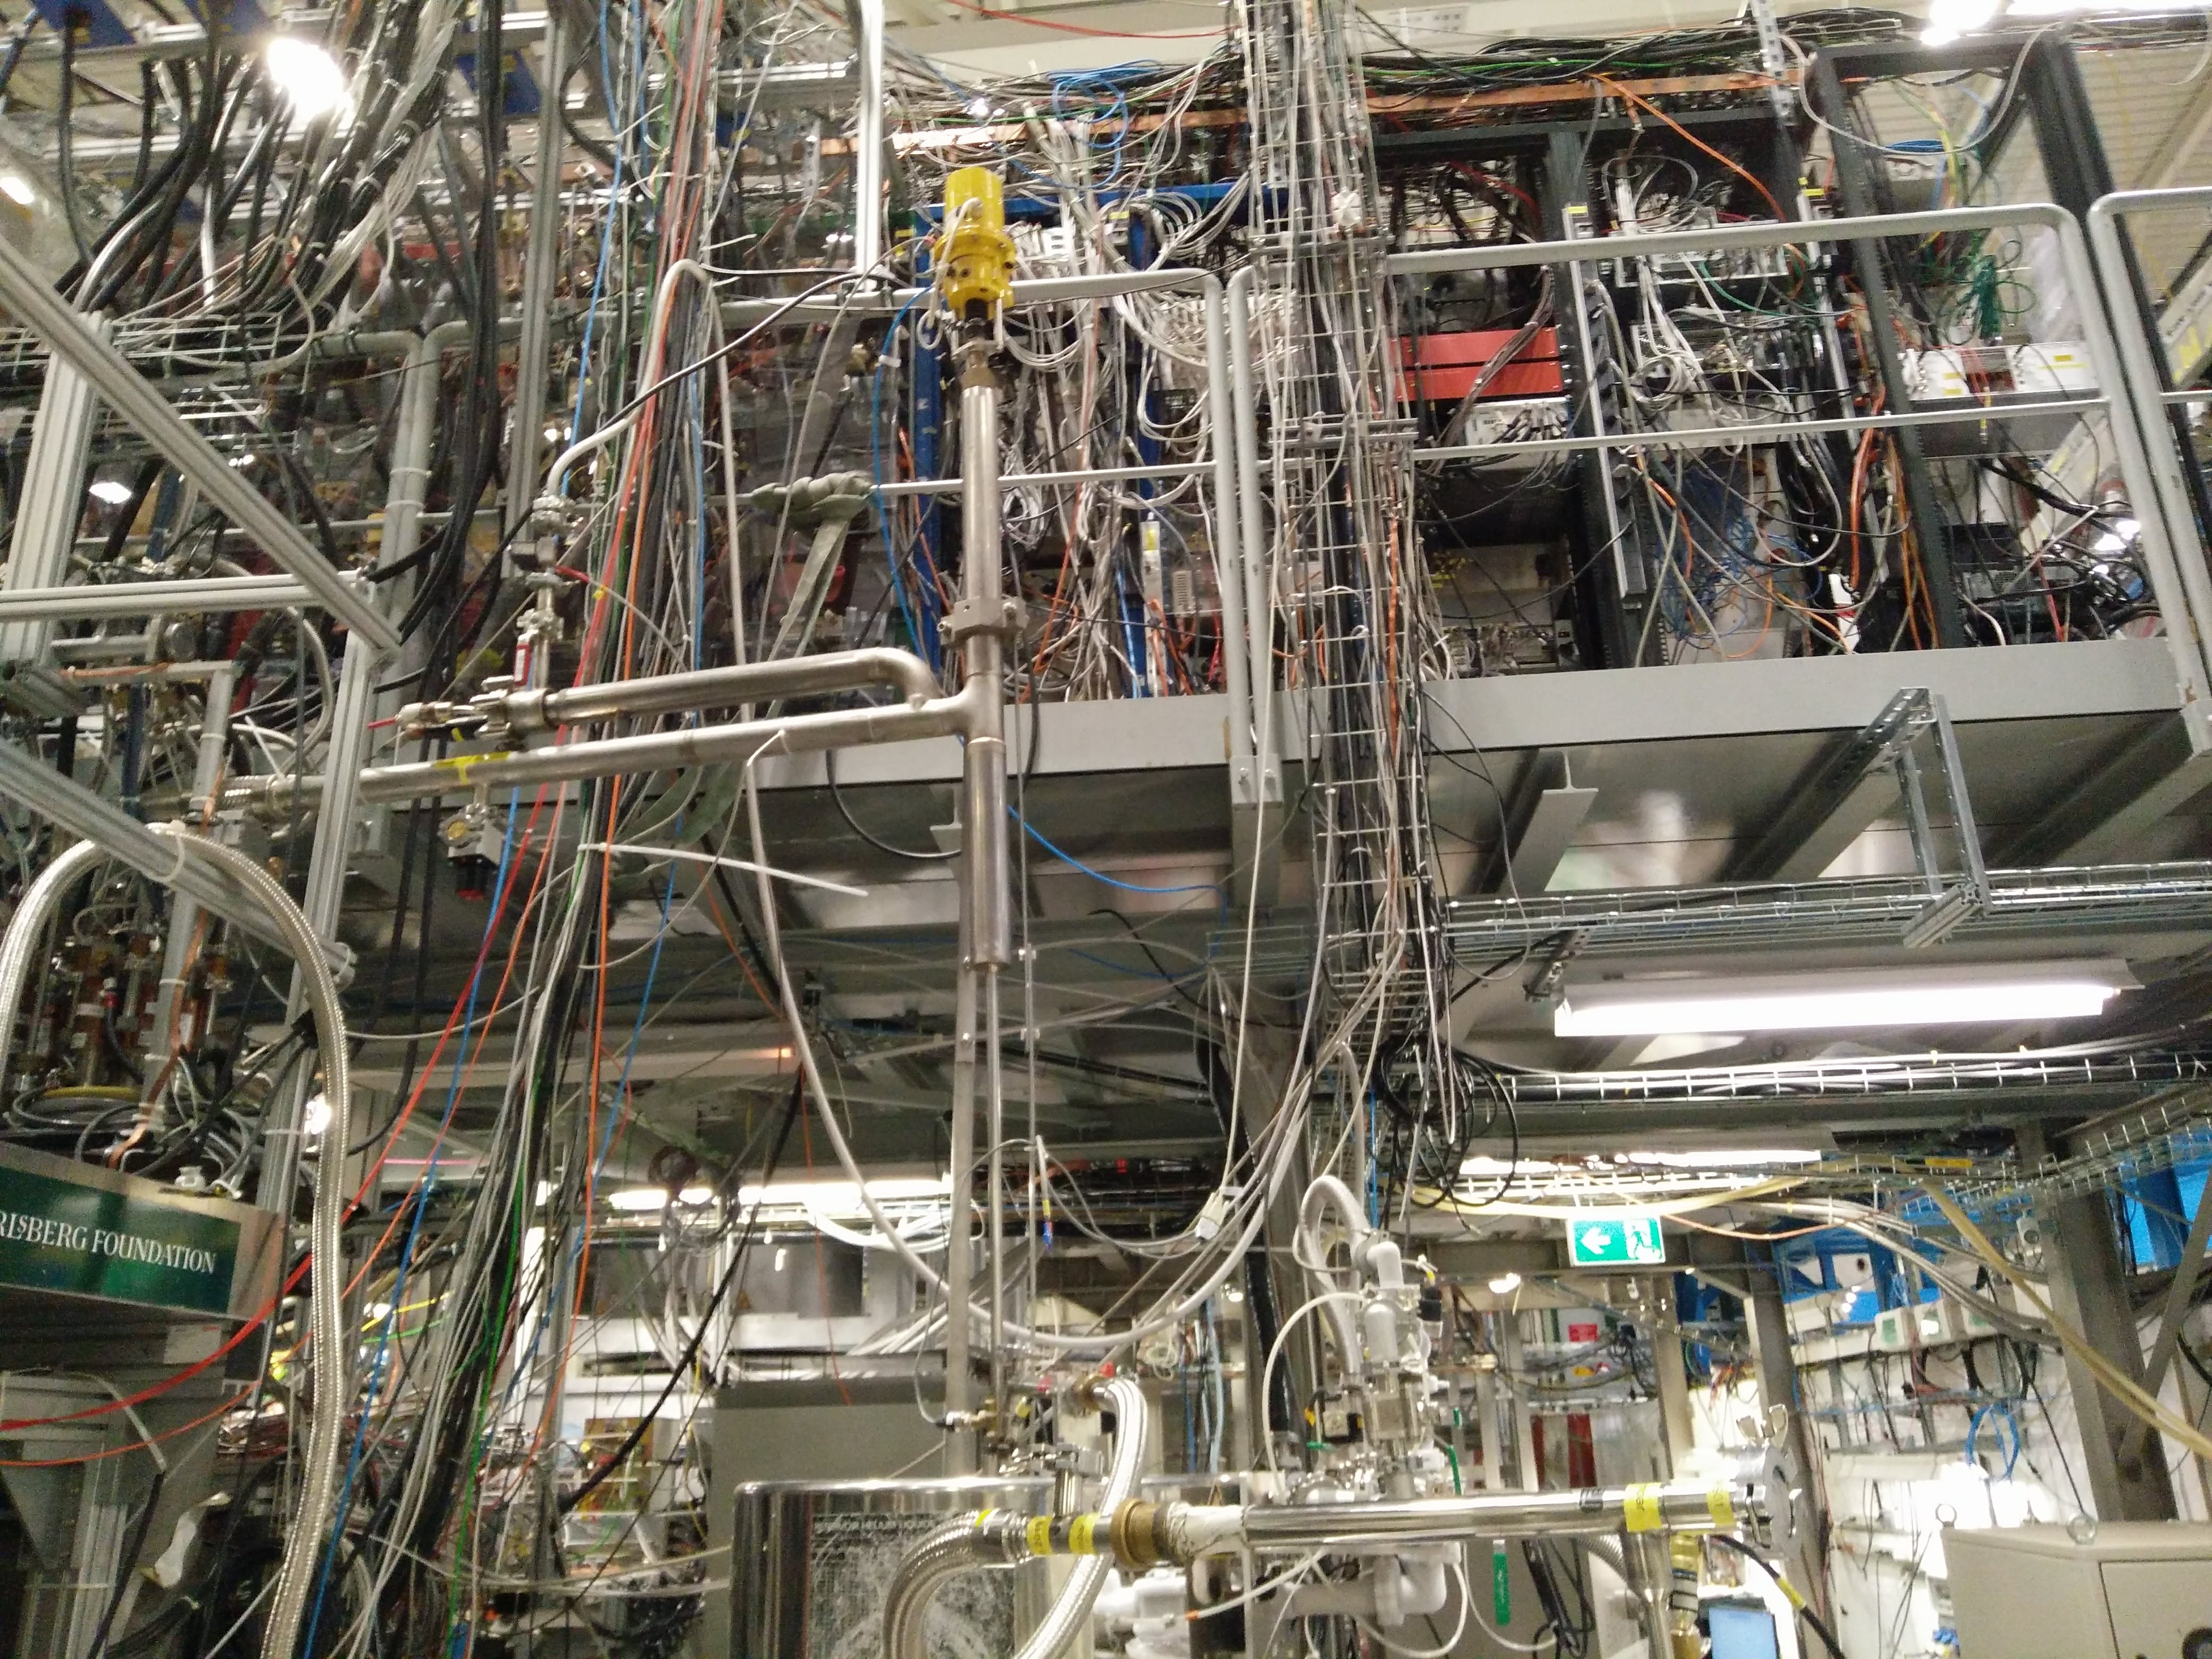
\includegraphics[height=60mm, width=75mm]{control_platform-1}
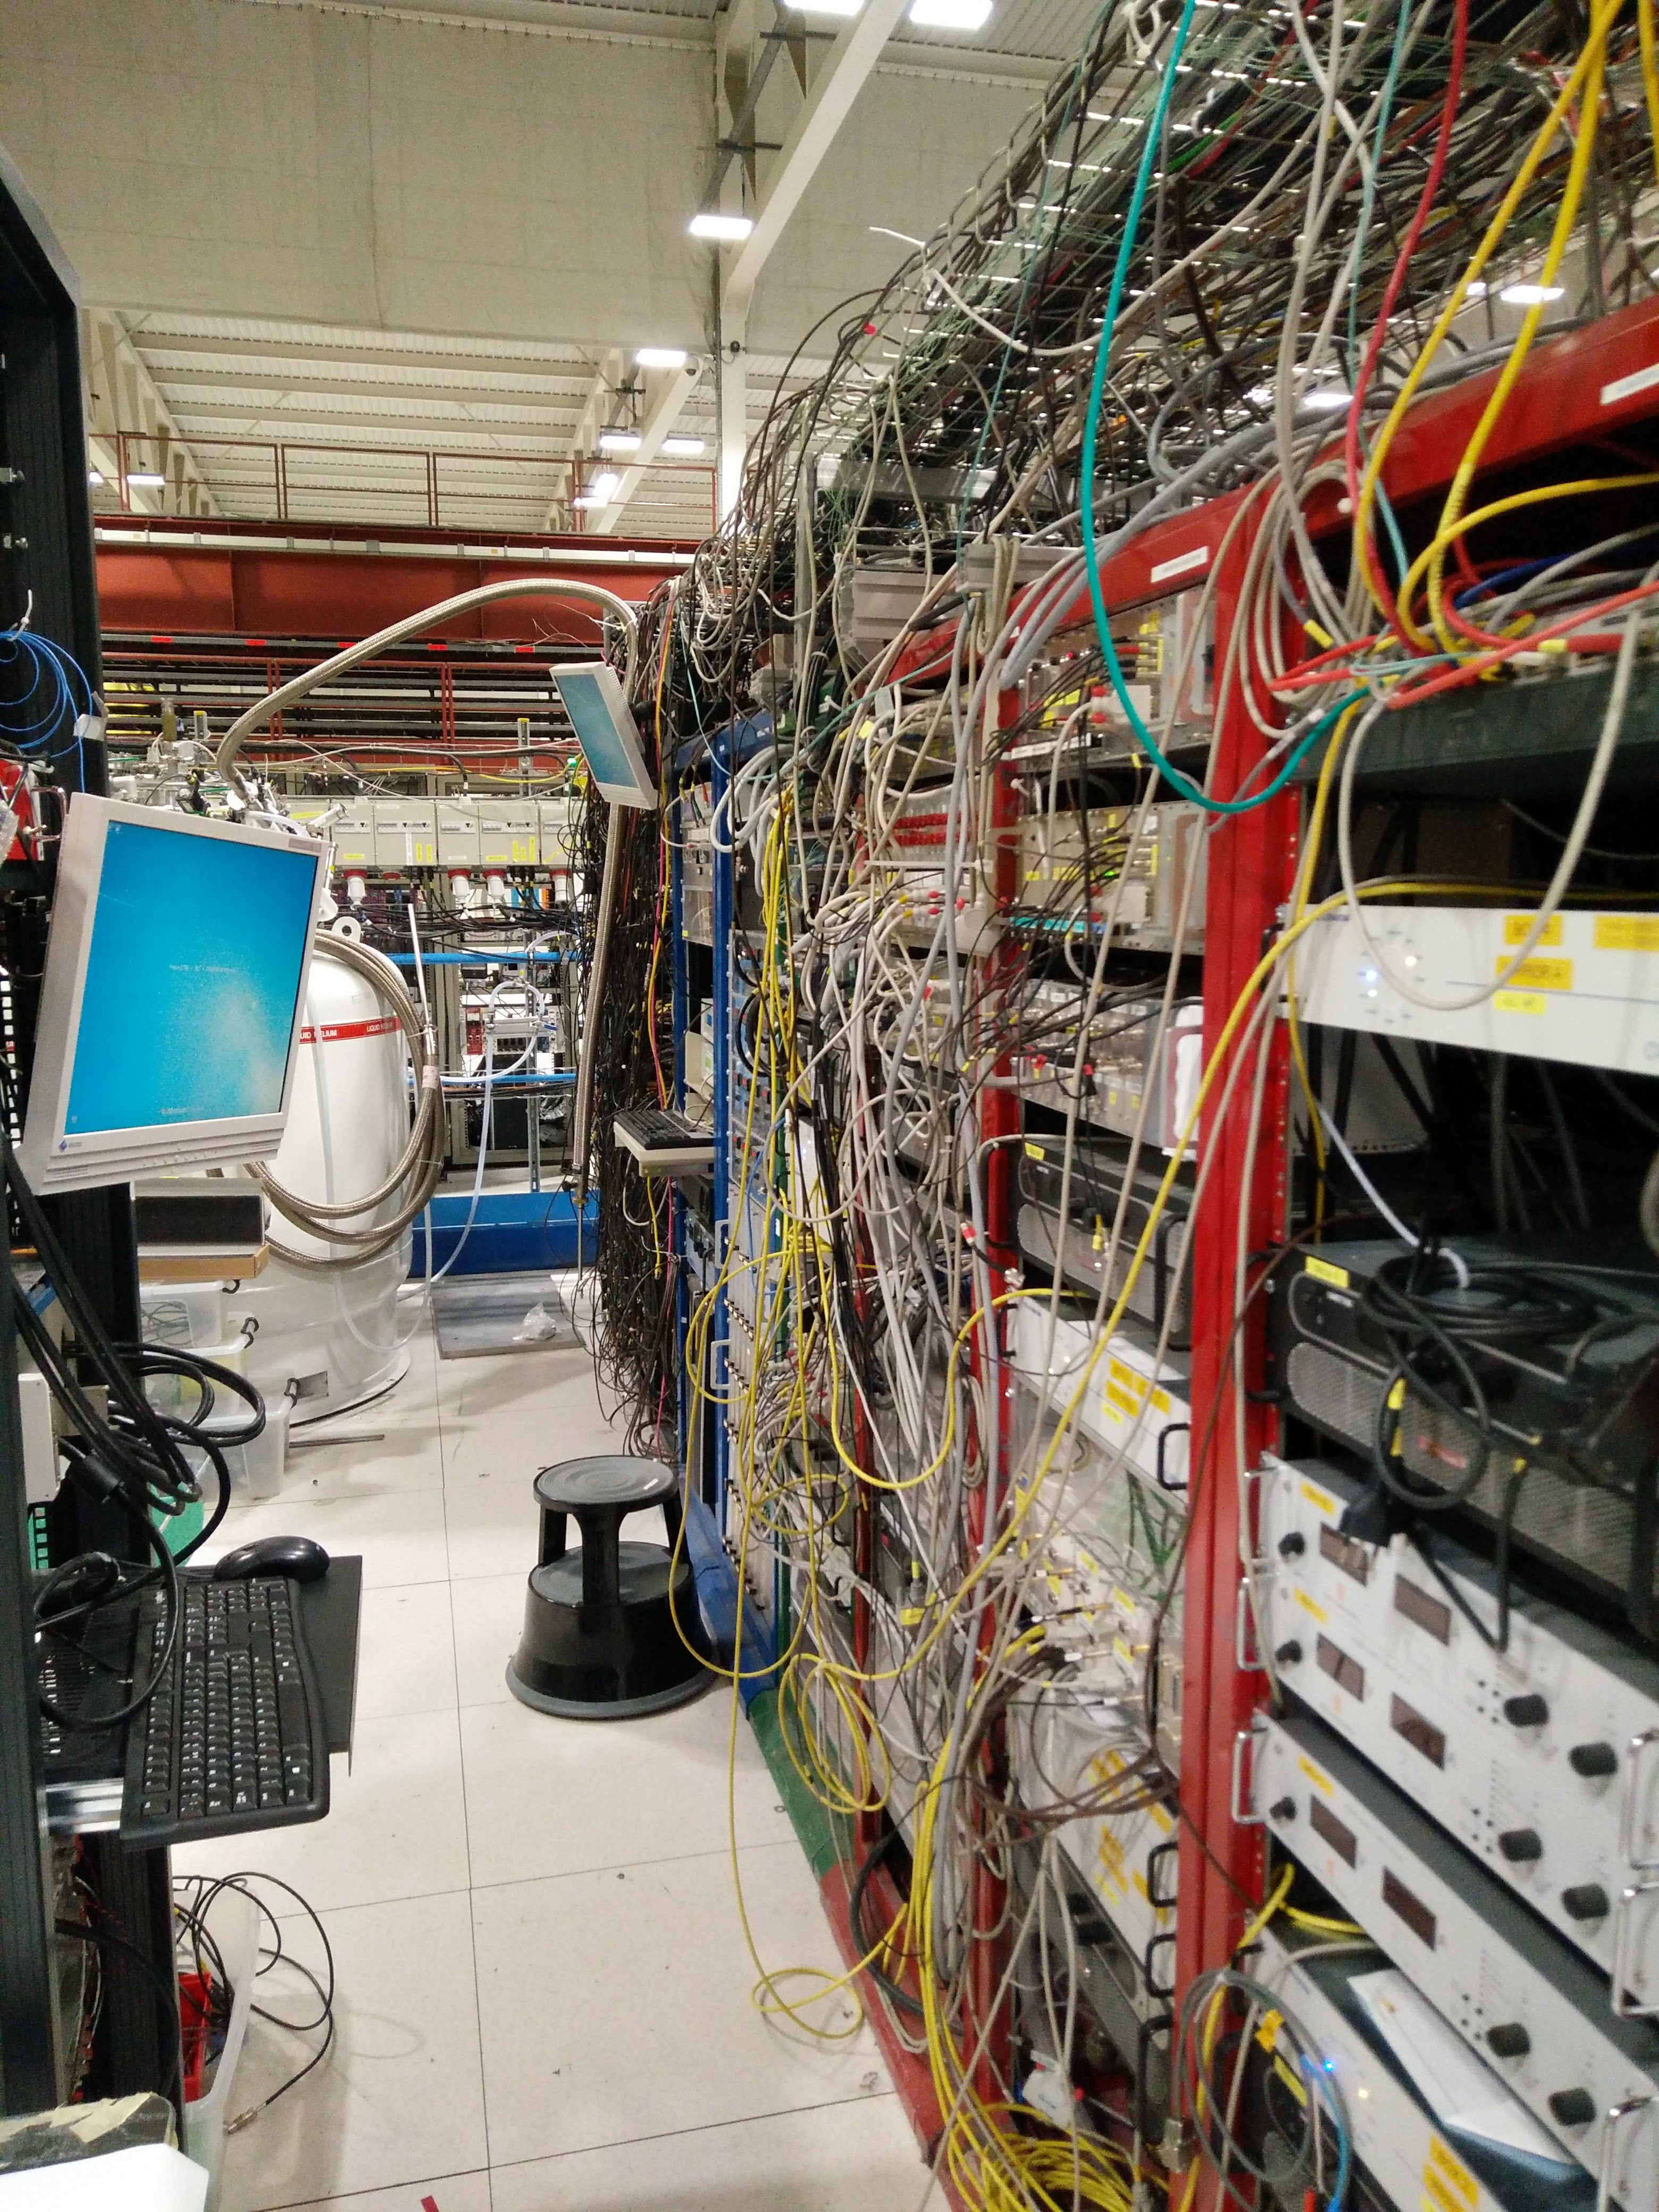
\includegraphics[width=45mm]{control_plattform2}
\caption{Control Platform}
\label{platform}
\end{figure}		
	
All of this computers have special cards installed on their motherboards ( for example NI PCI-6229 for analog inputs, NI PCI-6713 for analog outputs, NI PCI-8431 for RS 485 communications, NI PCI-8430 for RS 232 communication and many other cards). The user can control the experiment through these cards. The analog and digital signals which indicate the state of individual parts on experiment setup are collected by the input gates. Then after being evaluated in the control room, a proper signal will be sent by output gates to the experiment components (like vacuum pumps, valves, current of magnets, the electric potential on electrodes, etc).

\begin{figure}[h]
\centering
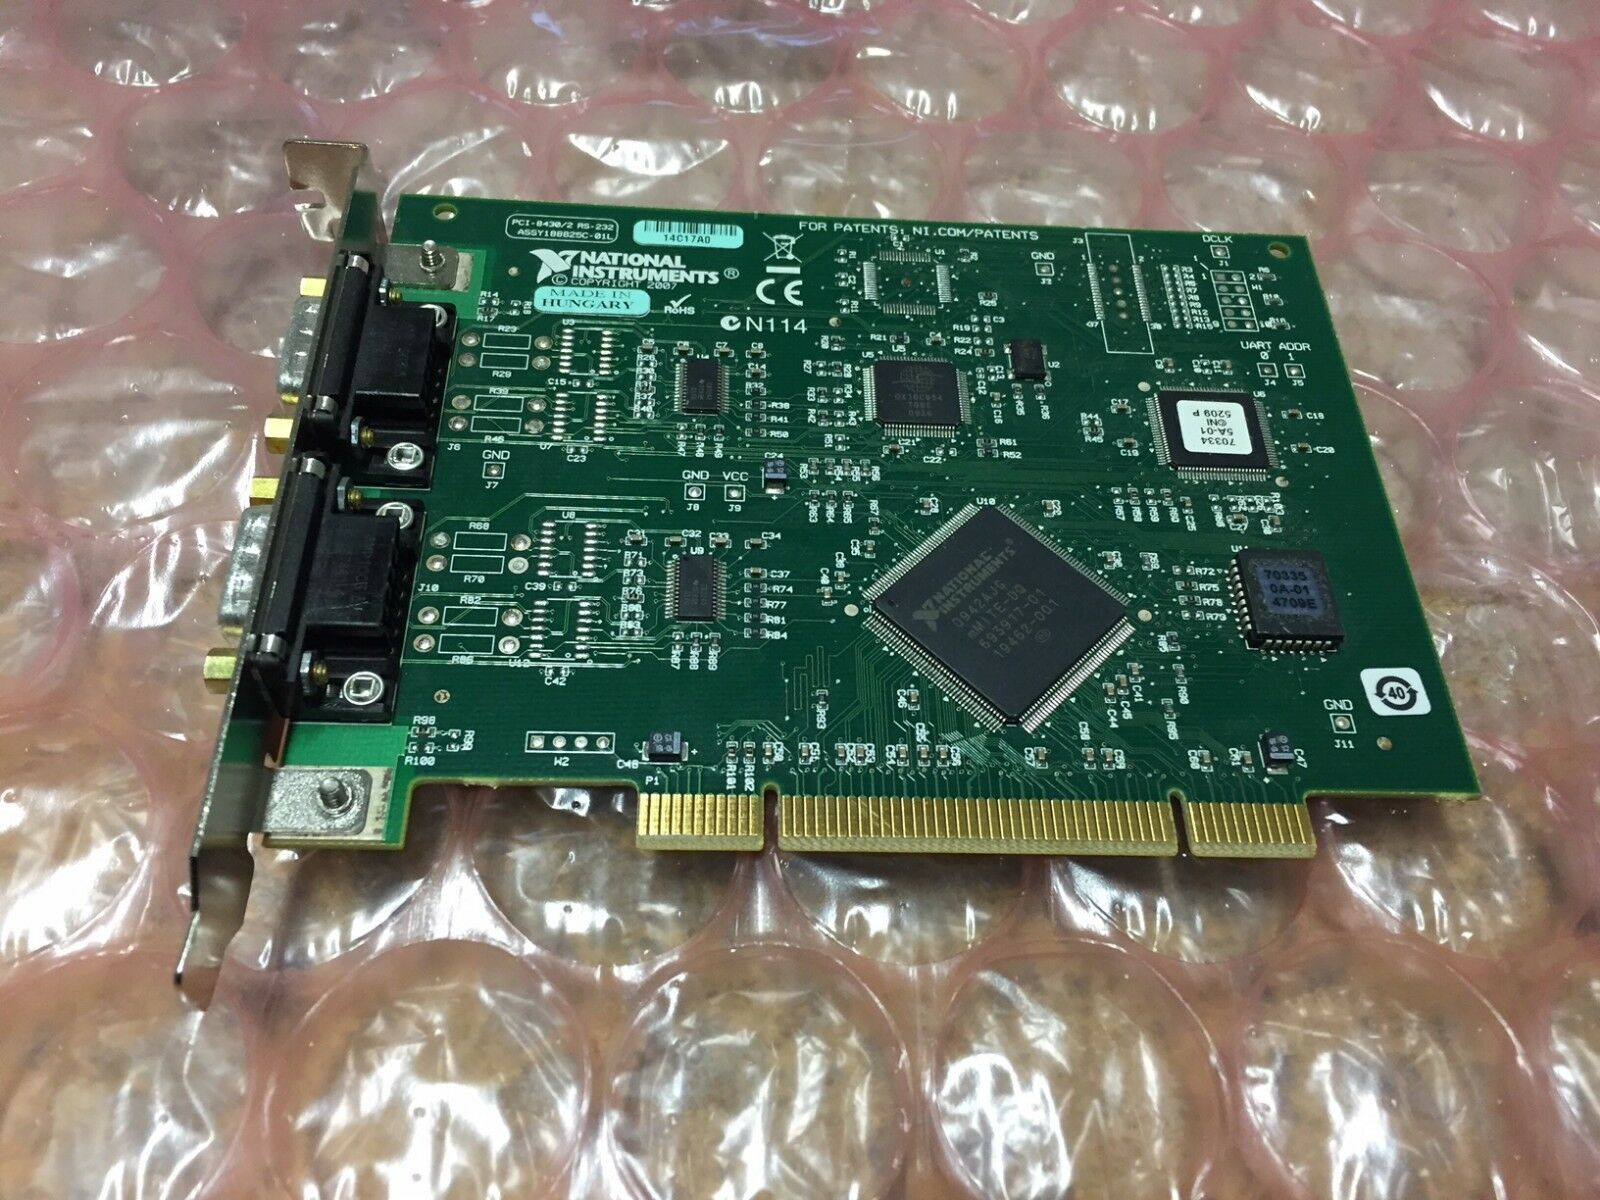
\includegraphics[width=40mm, height=50mm]{PCI_8430}
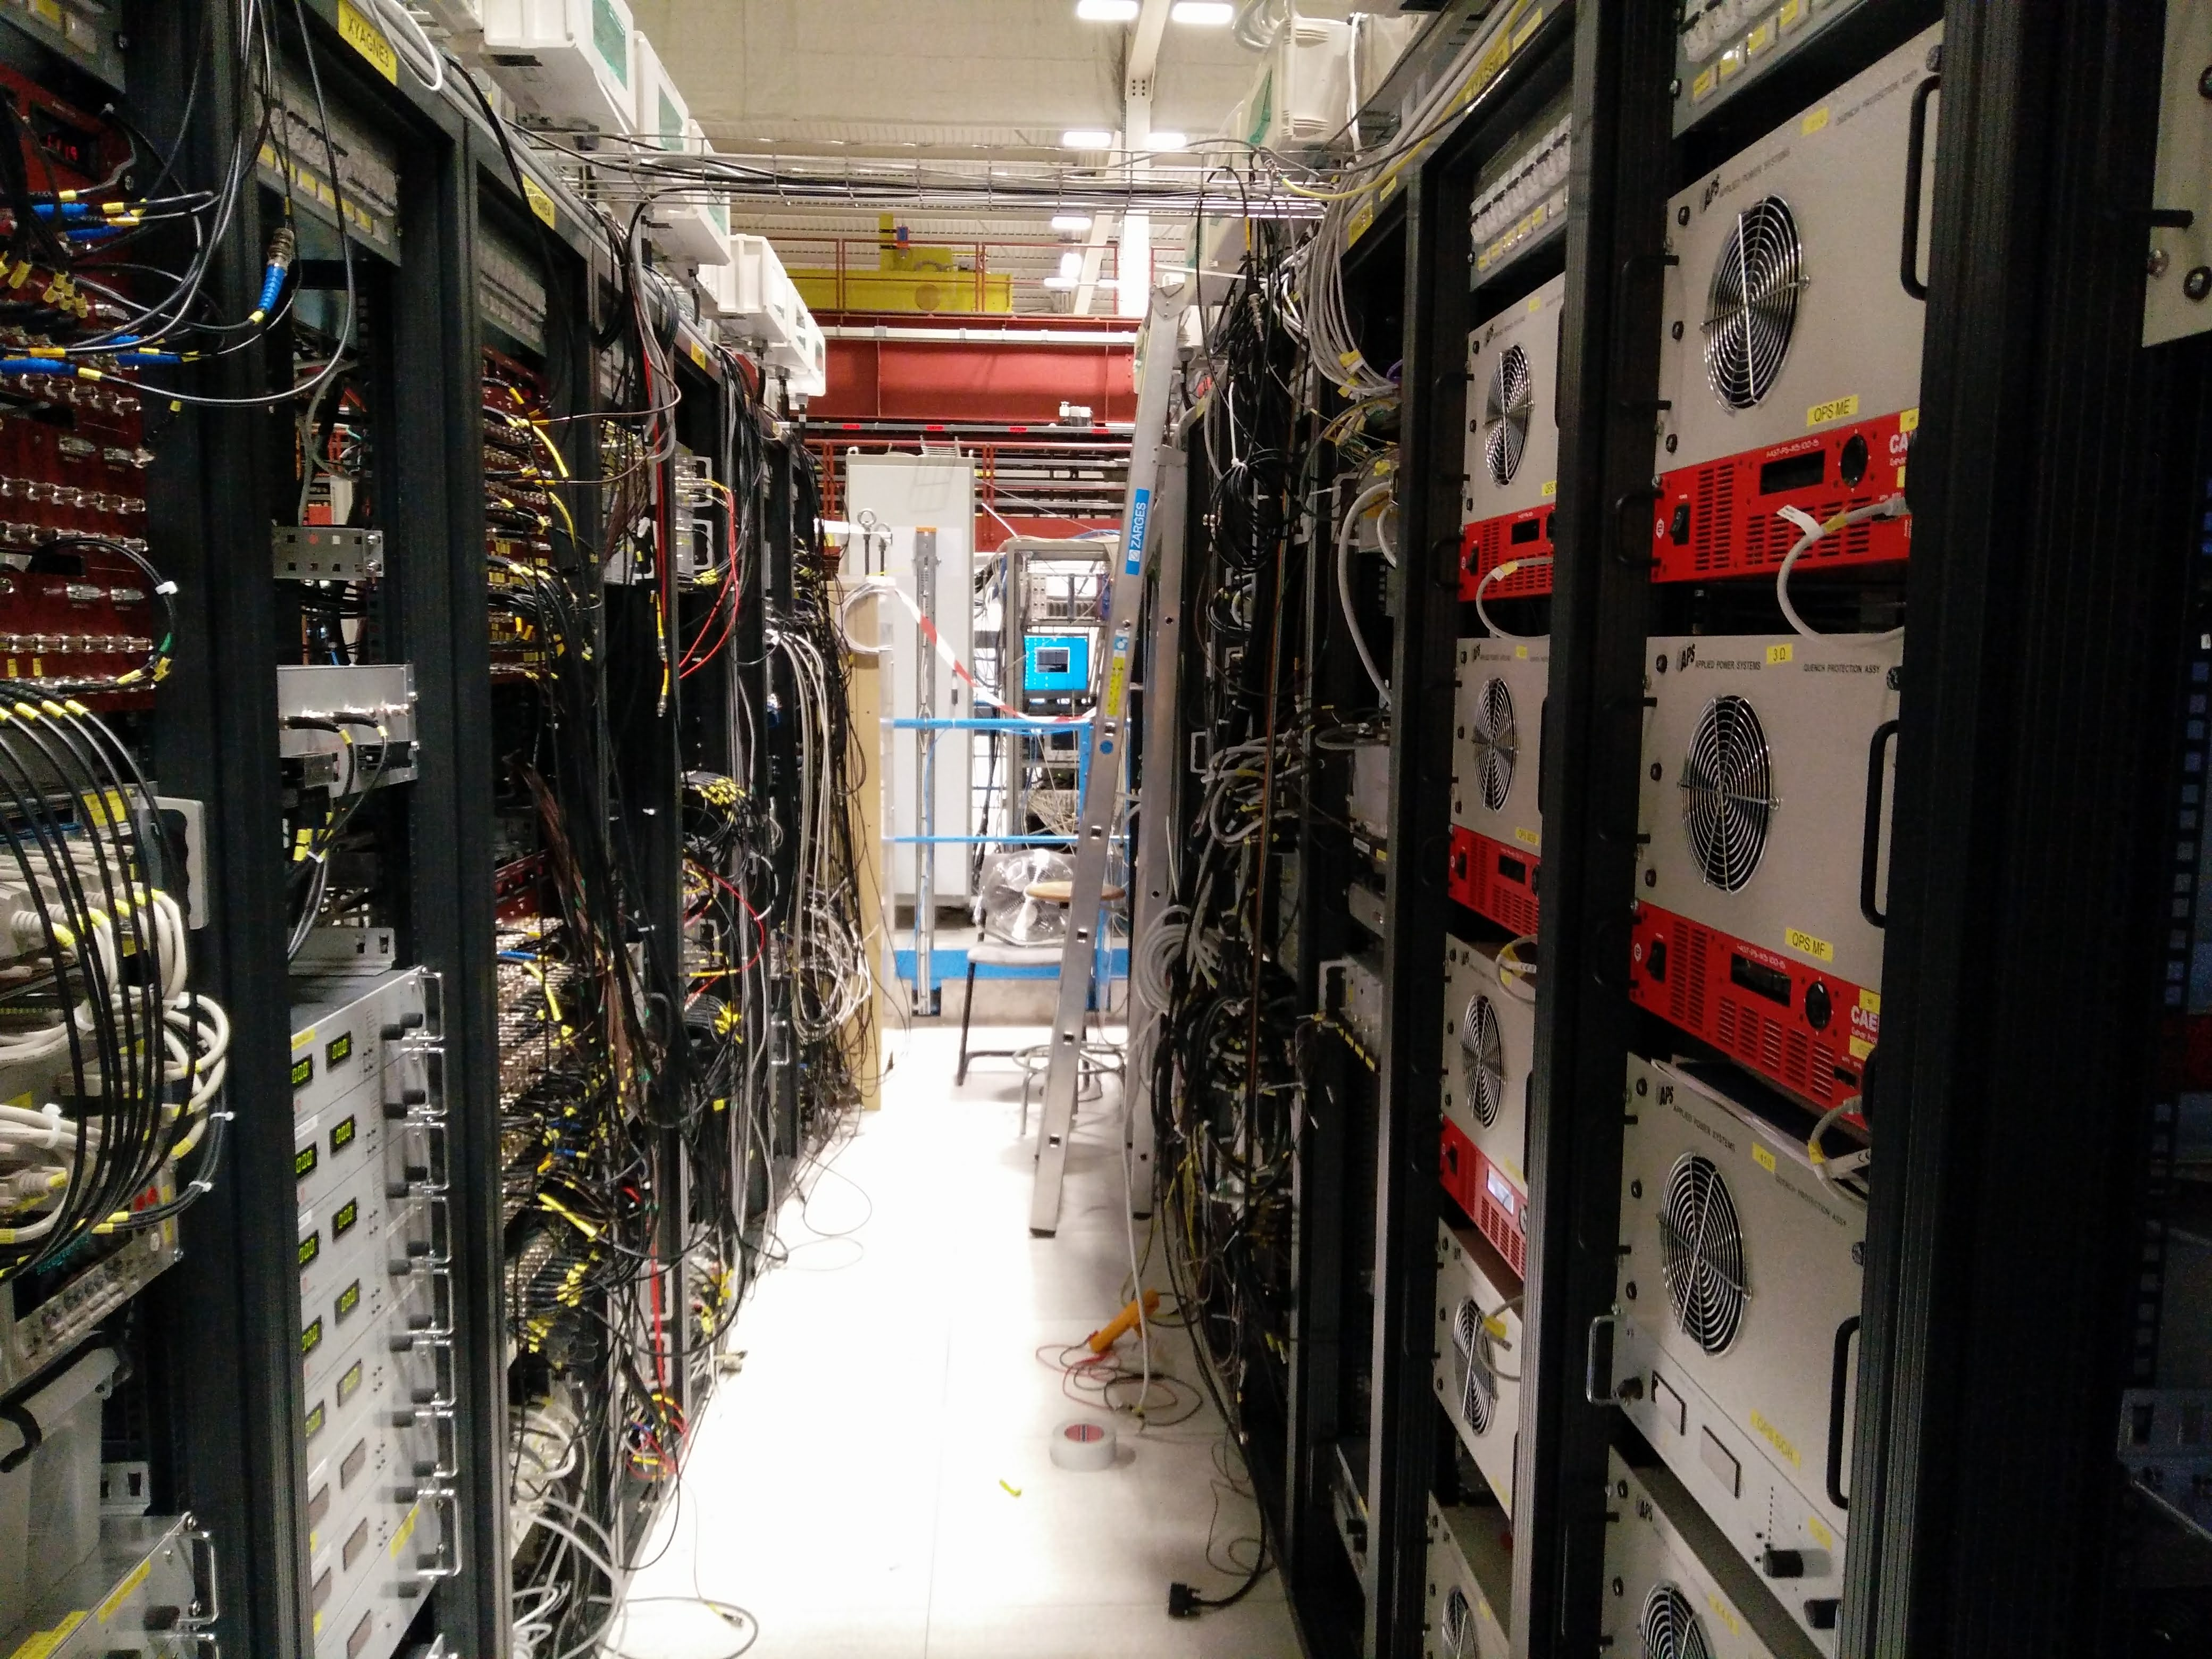
\includegraphics[width=80mm, height=50mm]{control_platform}
\caption{PCI 8430 card (left), and Computers on control platform equipted by DAQ cards (right) }
\end{figure}
	
\subsubsection{Virtual Instrument}

The Virtual Interface of VI that I have designed will contorl the valves, magnets, and vacuum pumps that are connected to the positron source and accumulator. You can see the front panel or the GUI of VI in figure \ref{VI}. 

The block diagram that controls this VI consists of three different sub-VIs. I have designed  block diagram to be modular, so my supervisor can add other control and options after my departure. each of these sub-VIs is for valves,vacuum pumps and positron stick section. These VIs must be fed by a number that indicates the state of a valve or vacuum pump to be On or Off, and by a string that the Icon of the elements in GUI is in it. The sub VI will browse the proper Icon considering the numeric input and will send the picture as Output. all of these elements are in an event structure to reduce the amount of CPU occupation. the reduction of CPU use is because the while loop containing the event structure will run for 1 time, just when you change the values of each event structure.

\begin{figure}[h]
\centering
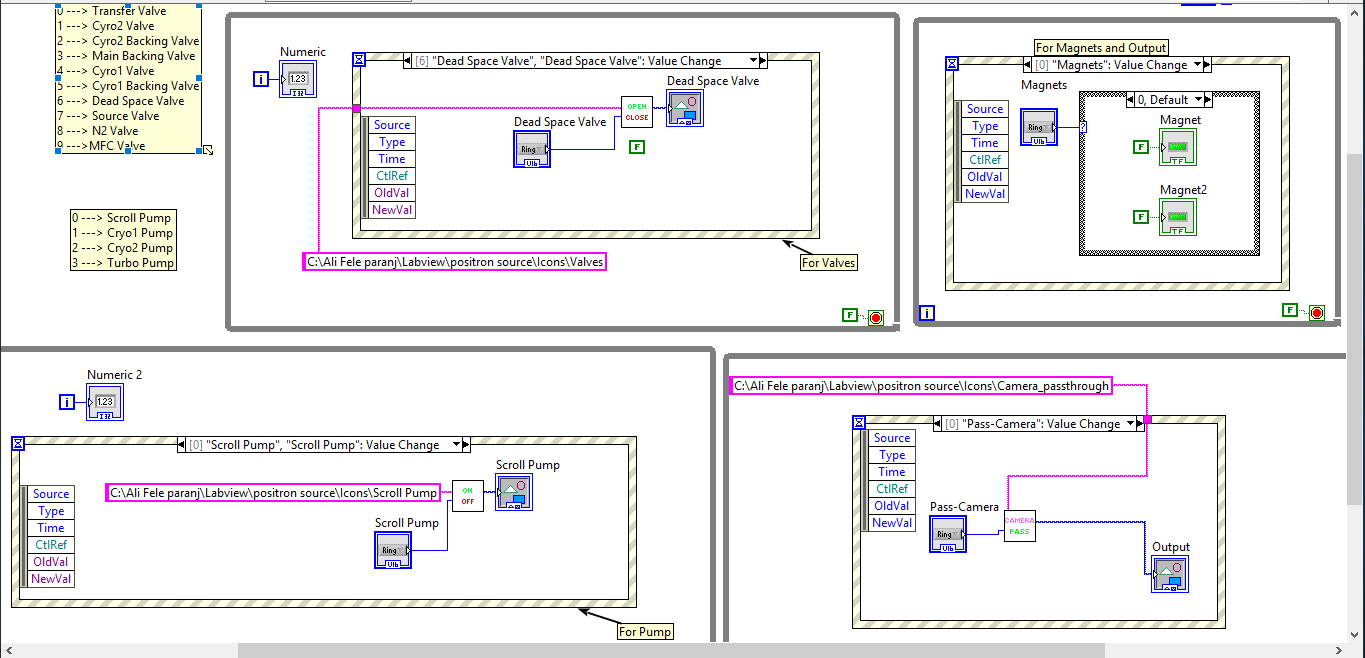
\includegraphics[scale=0.29]{Block-Diagram}
%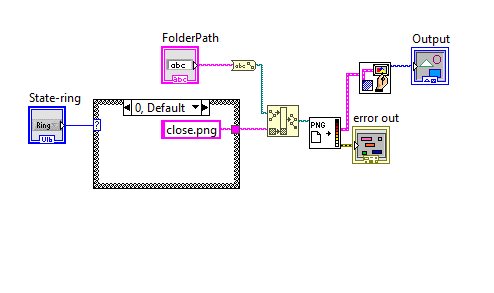
\includegraphics[scale=0.5]{SubVI}
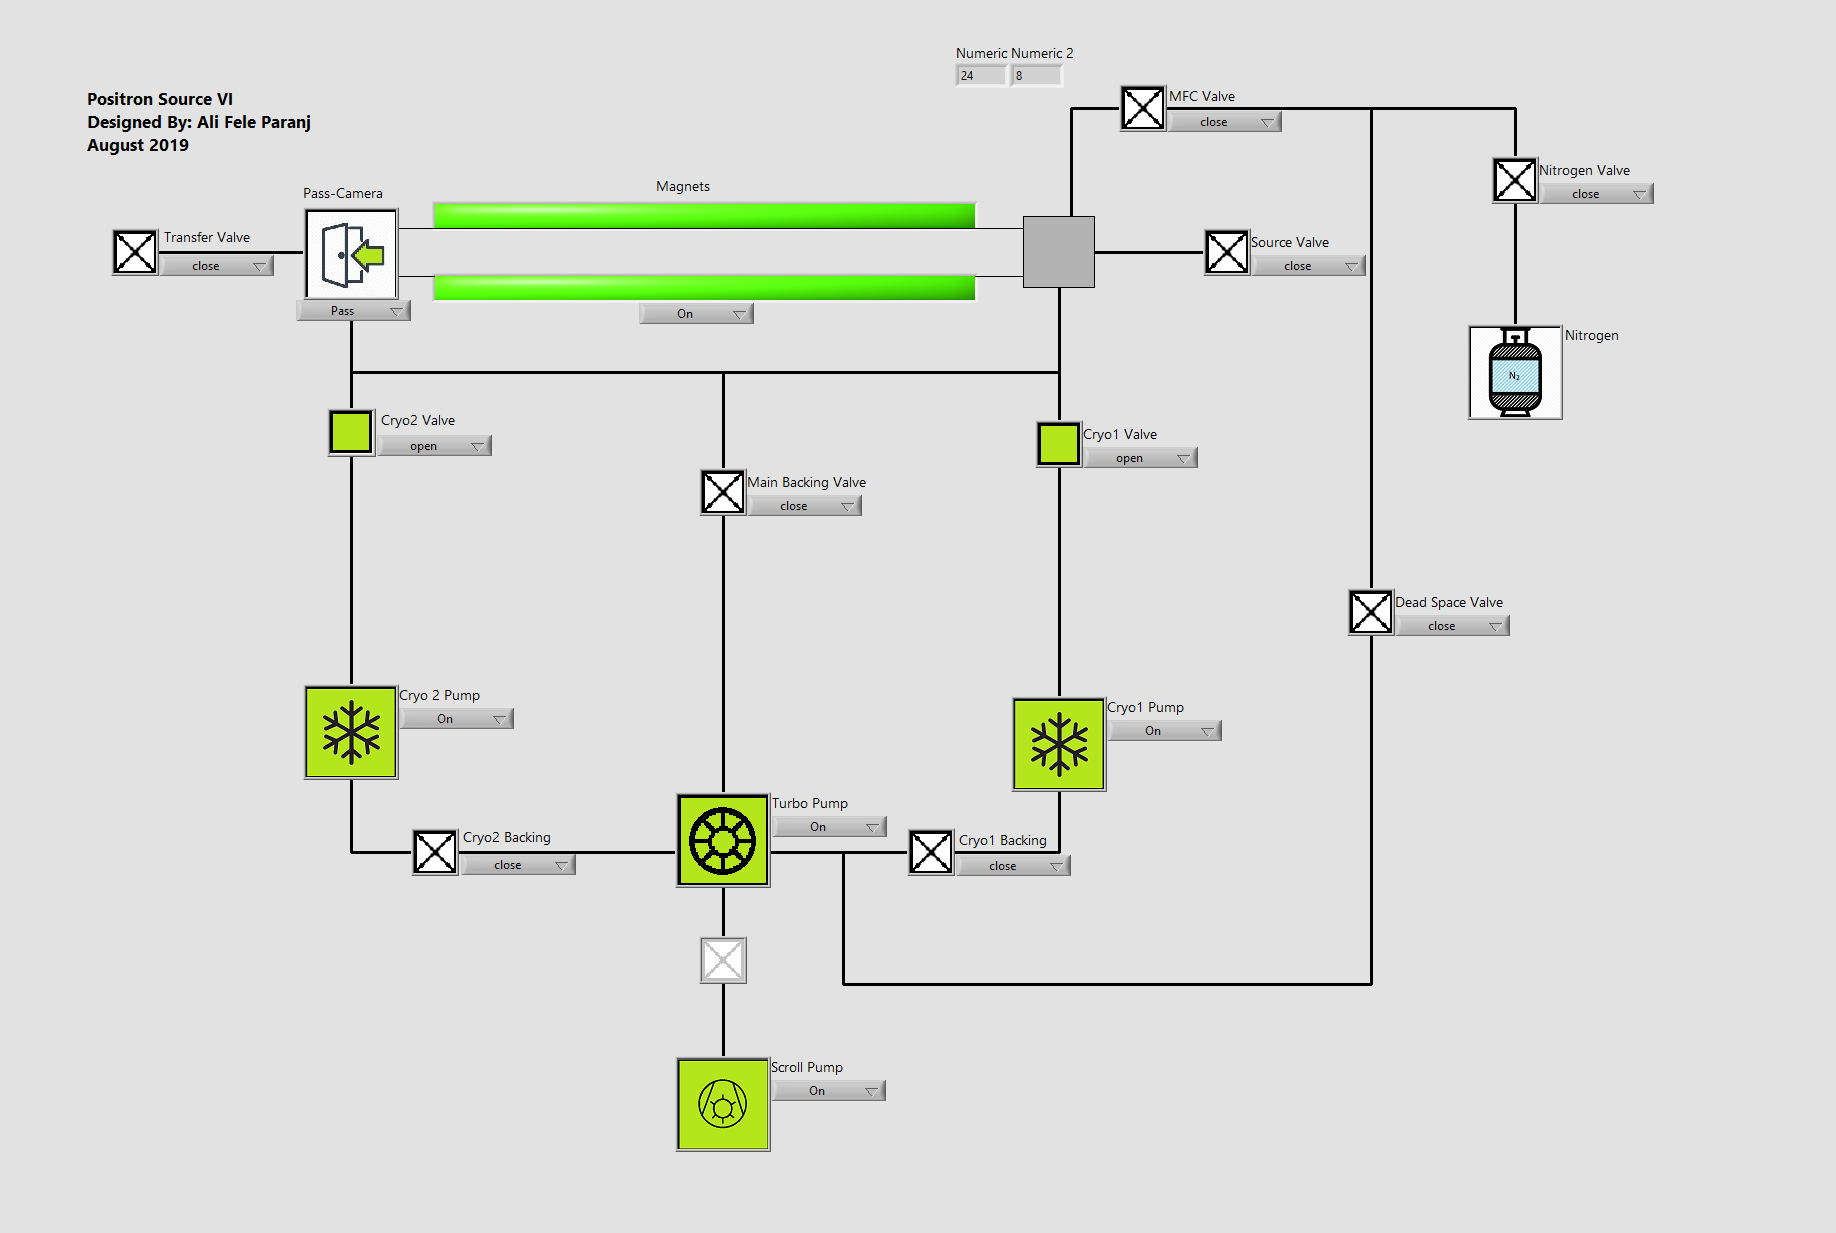
\includegraphics[scale=0.22]{InterFace}
\caption{First: the Block Diagram of VI, Second: the user Interface}
\label{VI}
\end{figure}

\subsection{Compact Rio Upgrade}
As mentioned before, handling advanced experiments requires advanced electronics. As time passes, the electronics and computers get more powerful. So one of the most important 'Must do's for every experiment is upgrading the electronics to the last technologies. ALPHA was born in 2005 and since that day many updates had been done on setup and computers. A part of the new update is transferring the old computers with DAQ cards to professional Compact Rio computers that are designed mainly for Experimental control and data acquisition purposes. In more details, CompactRIO (or cRIO) is a real-time embedded industrial controller made by National Instruments for industrial control systems. The CompactRIO is a combination of a real-time controller, reconfigurable IO Modules (RIO), FPGA module and an Ethernet expansion chassis.(figure \ref{crio}). In these computers, we use DAQ modules instead of DAQ cards. This will make the control platform very compact and of course more professional. In some of the modules that we use with these computers, we need to separate the data lines in order to use them individually. for this purpose, we need to design a printed circuit board (PCB), that maps every pin on D-subminiature connector to individual Lemo connectors.

\begin{figure}[h]
\centering
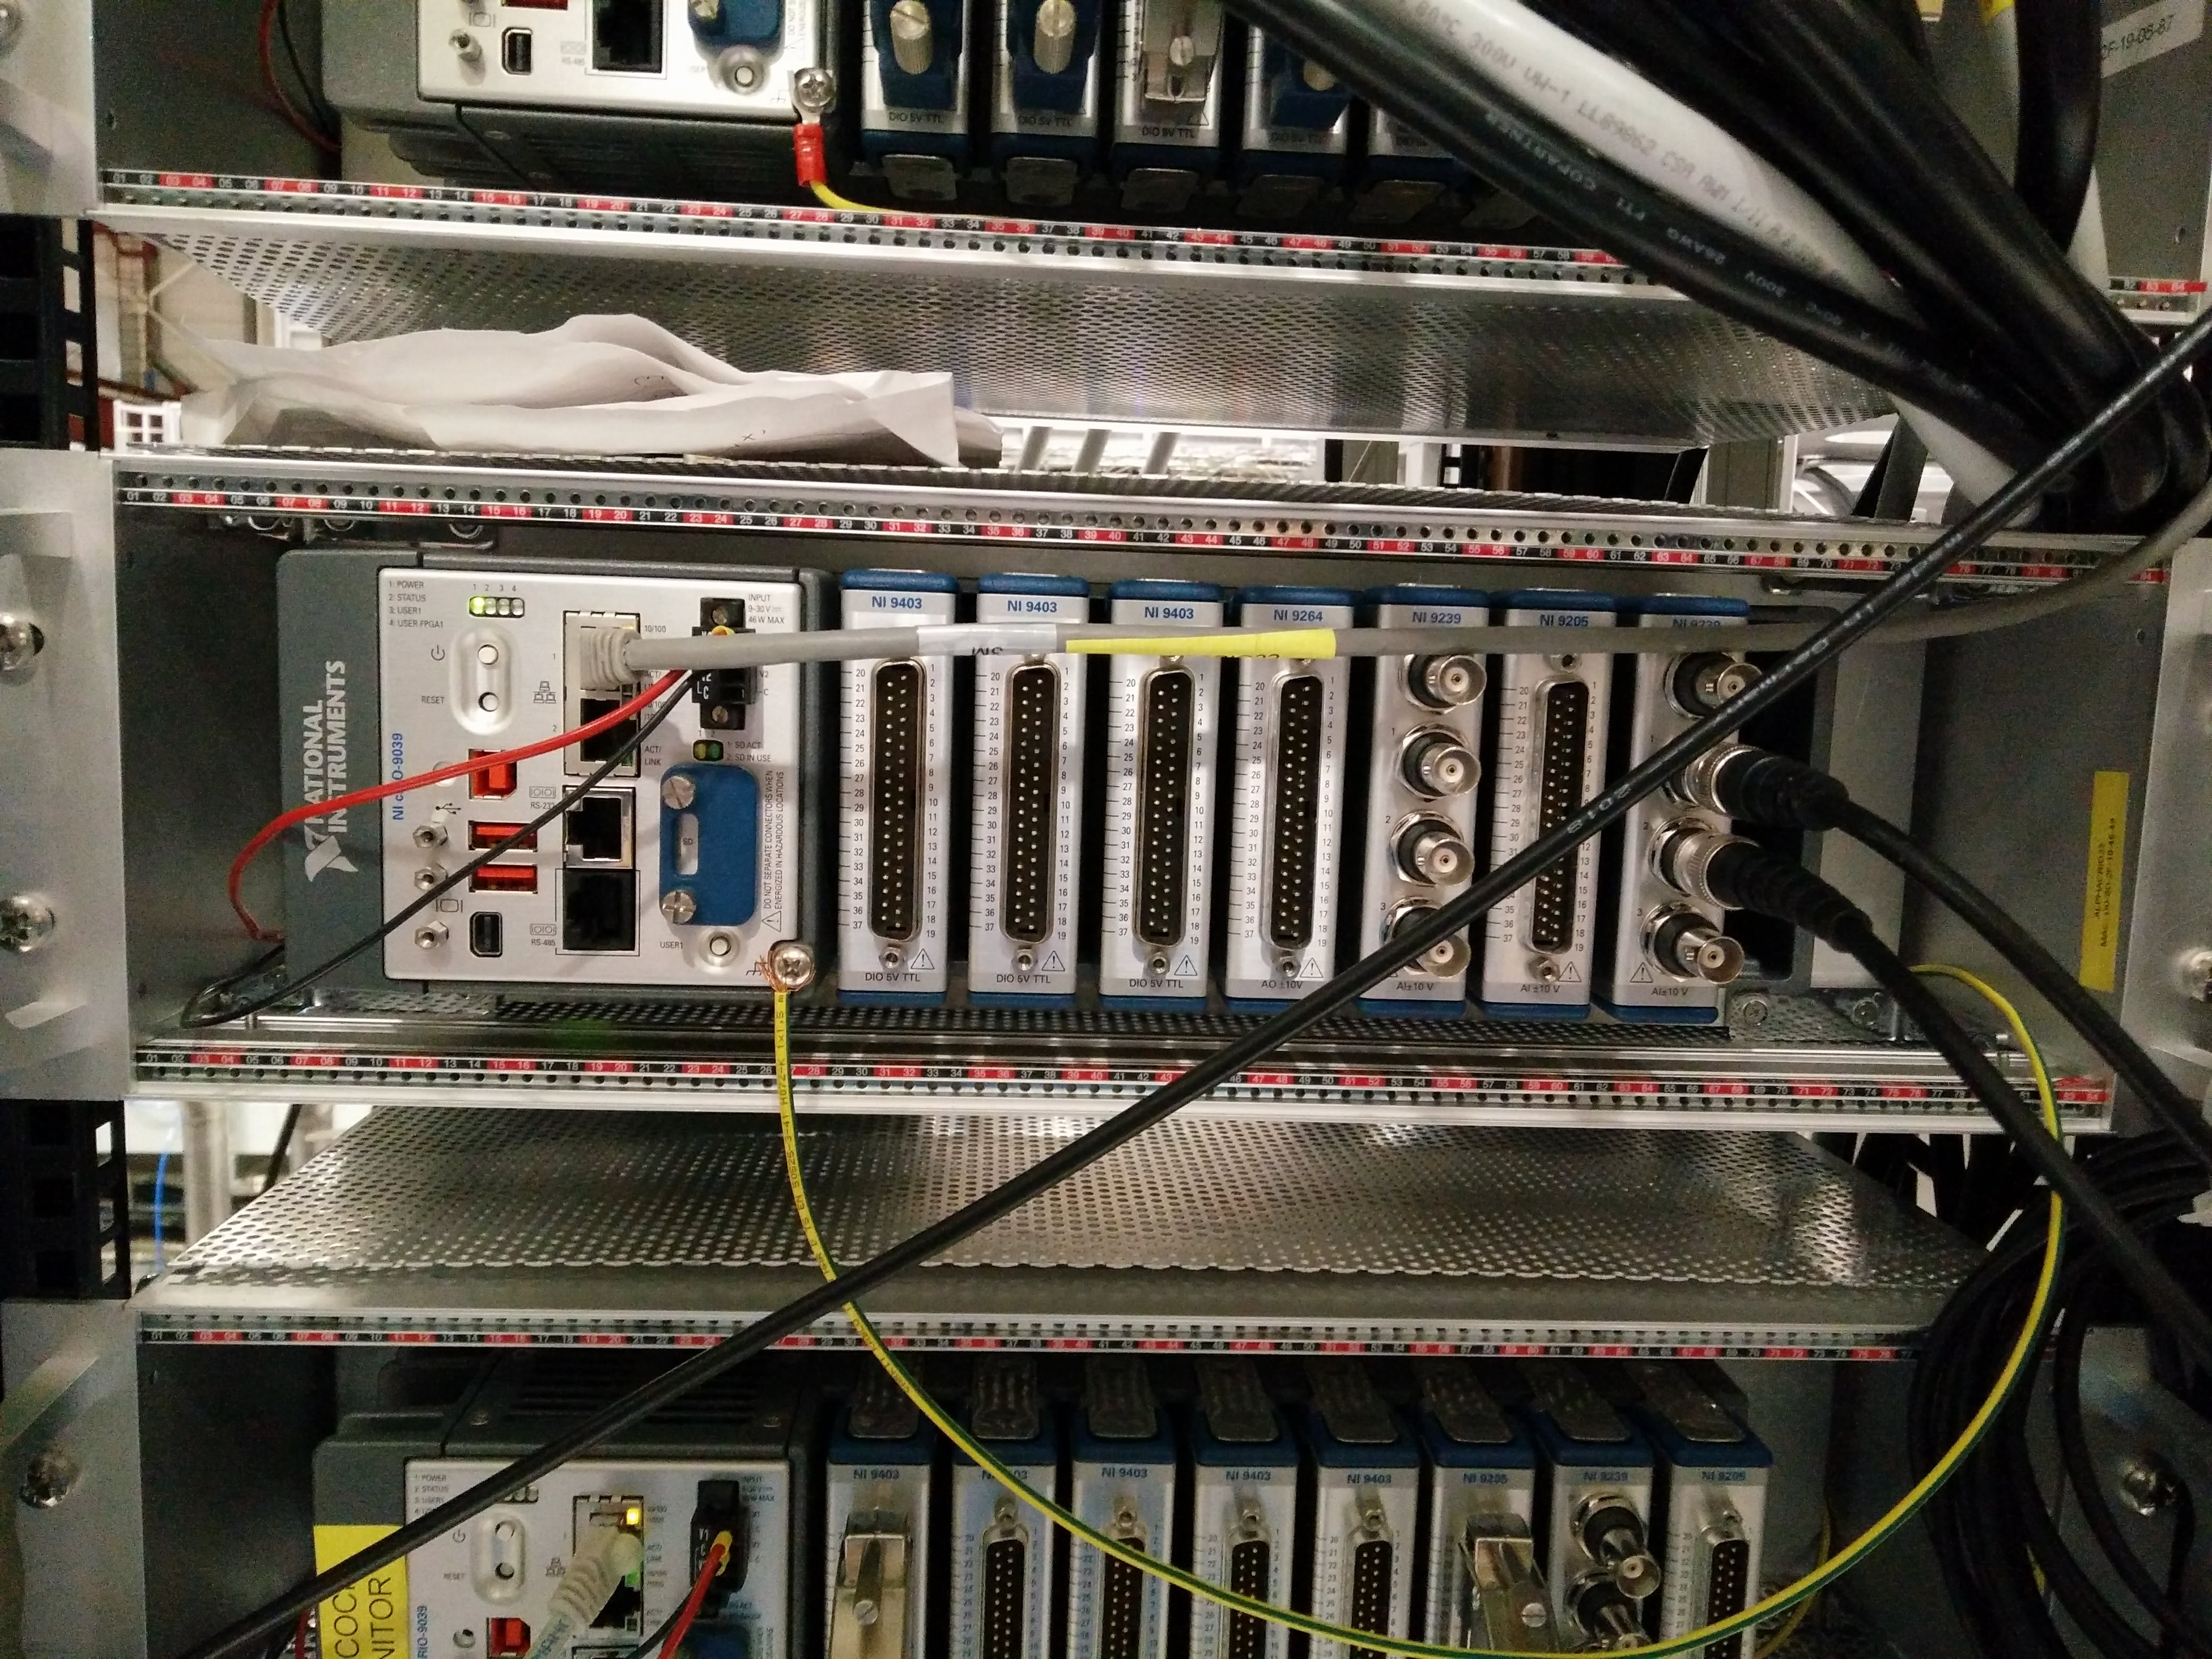
\includegraphics[width=105mm, height=60mm]{crio}
\caption{Compact Rio}
\label{crio}
\end{figure}

\subsubsection{PCB and Front Panel Design}
In this project, I designed PCBs using "Altium design' software. this PCBs connect the D-subminiature connector to individual Lemo Connectors. Throughout this report, I will call these PCBs "Data Line Separator" or DLS. We had four different types of modules, so I needed to design four different PCBs.
The modules were NI9264, NI9401, NI9403, NI9205 (see figure \ref{module}). these modules are digital and analog modules that are connected to a compact Rio system to control the experiment apparatus. For example, one can control valves, vacuum pumps, mass flow rate controllers, etc. These are done by using the LabVIEW interface which I worked with and designed an interface in other projects that I described earlier. You can find mentioned modules in figure \ref{module}

\begin{figure}
\centering
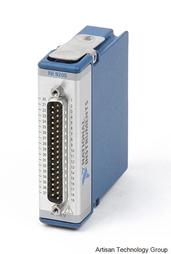
\includegraphics[width=27mm, height=24mm]{ni9205}
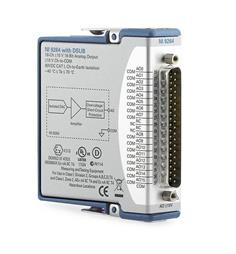
\includegraphics[width=27mm, height=24mm]{ni9264}
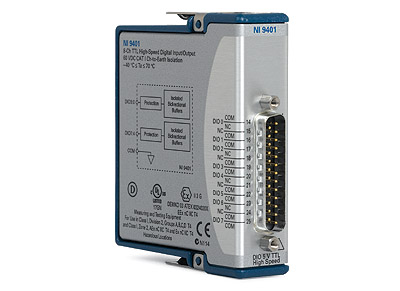
\includegraphics[width=38mm, height=24mm]{ni9401}
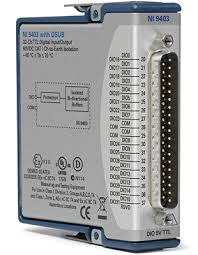
\includegraphics[width=24mm, height=24mm]{ni9403}
\caption{(left to right) NI 9205, NI 9264, NI 9401, NI 9403}
\label{module}
\end{figure}

As I said before, for complicated experiments there is a control platform that controls the parameters of the experiment. 
These platforms are where the Compact Rio will sit at. Each compact Rio will be held at chassis and these chassis will be held horizontally on top of each other. so to keep everything clean, we need to design front panels that can mount on chassis, and screw the PCBs to them. I did so for each of the modules and you can see the front panel of the NI9205 module in figure \ref{NI}. You can find full documents at my GitHub repository for CERN as well.


\begin{figure}[h]
\centering
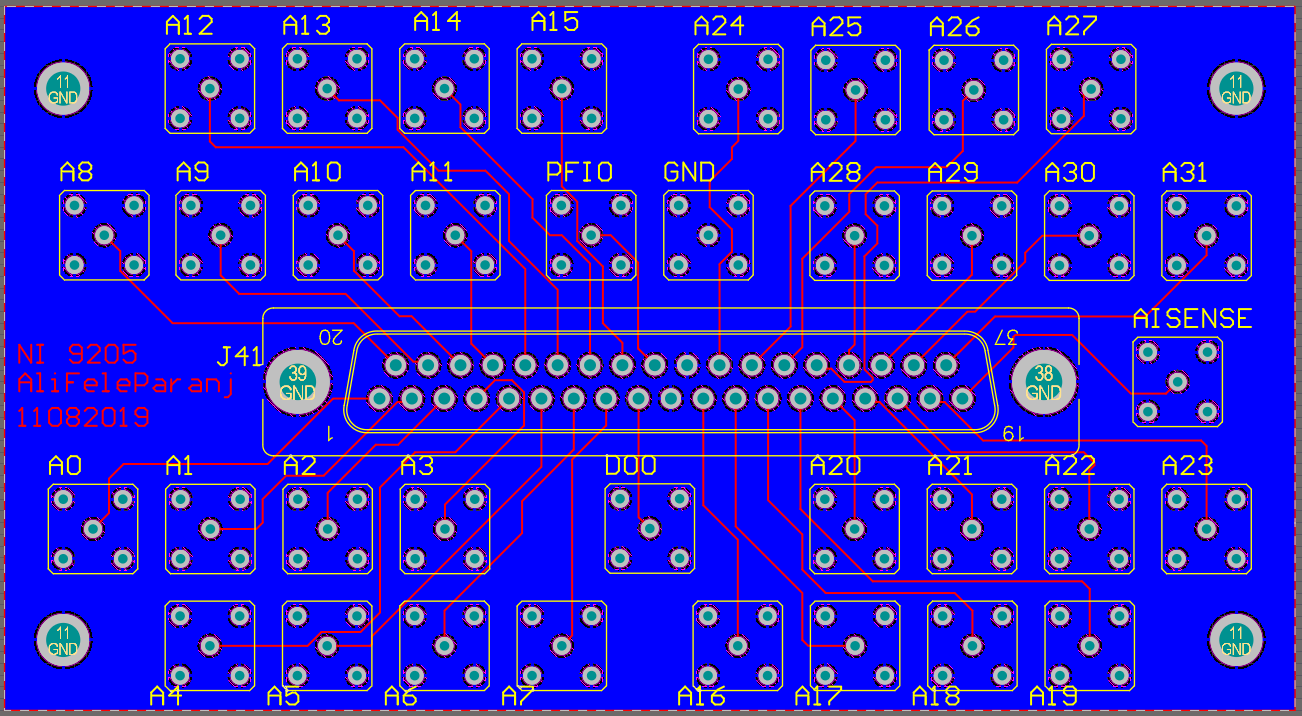
\includegraphics[width=50mm, height=28mm]{ni9205_pcb}
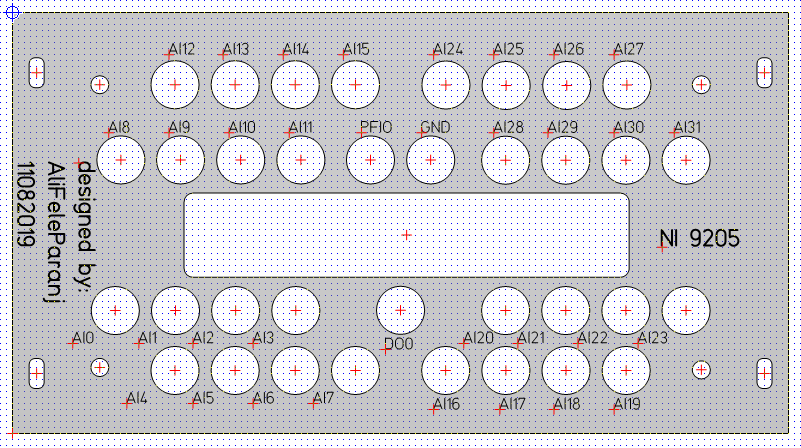
\includegraphics[width=50mm,
height=28mm]{ni9205panel}
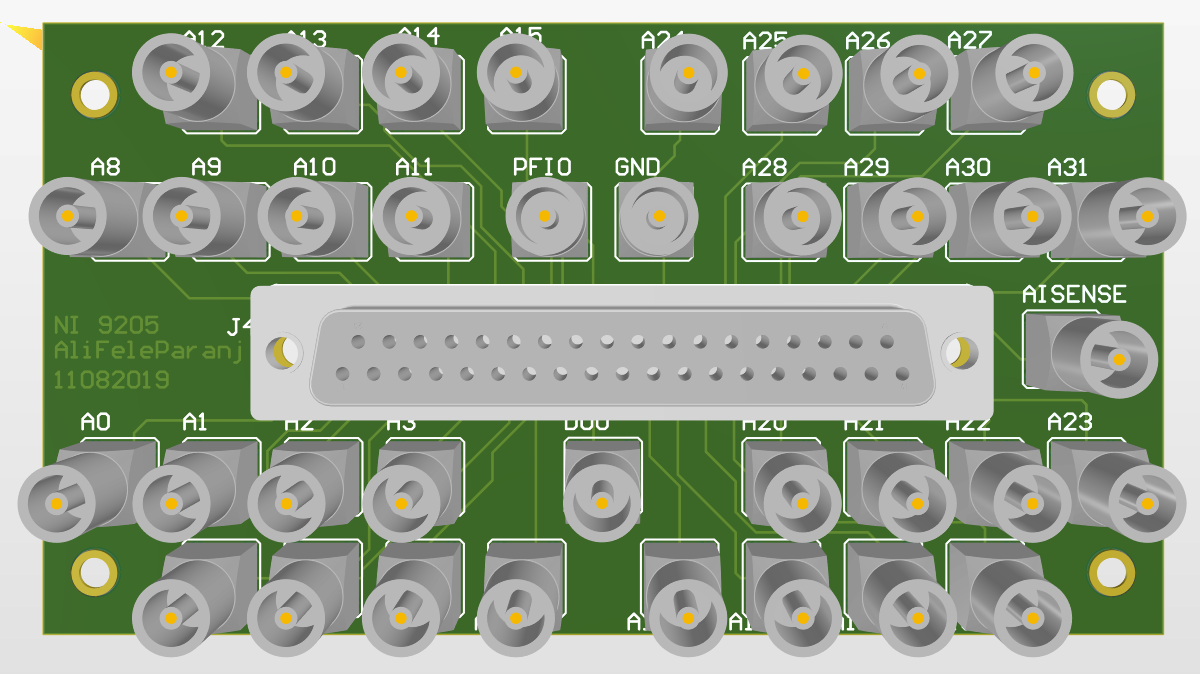
\includegraphics[width=75mm,
height=37mm]{ni9205_3d}
\caption{First: DLS designed for NI9205 module, Second: 3D model of DLS, Third: Front Panel Designed for NI9205 DLS}
\label{NI}
\end{figure}


\subsection{Full Simulation}
\label{clus}
‌Simple simulations are very useful when you want to evaluate your estimates using the minimum computation resources. But after finding the rough simulations satisfactory, you need to improve your simulated model and add more details to it. In the simple simulation of buncher, we find out that buncher works pretty well in bunching the expanding beam. So we decided to add more details to our simulation and simulate the full setup of magnets and beamline.

\begin{figure}[h]
\centering
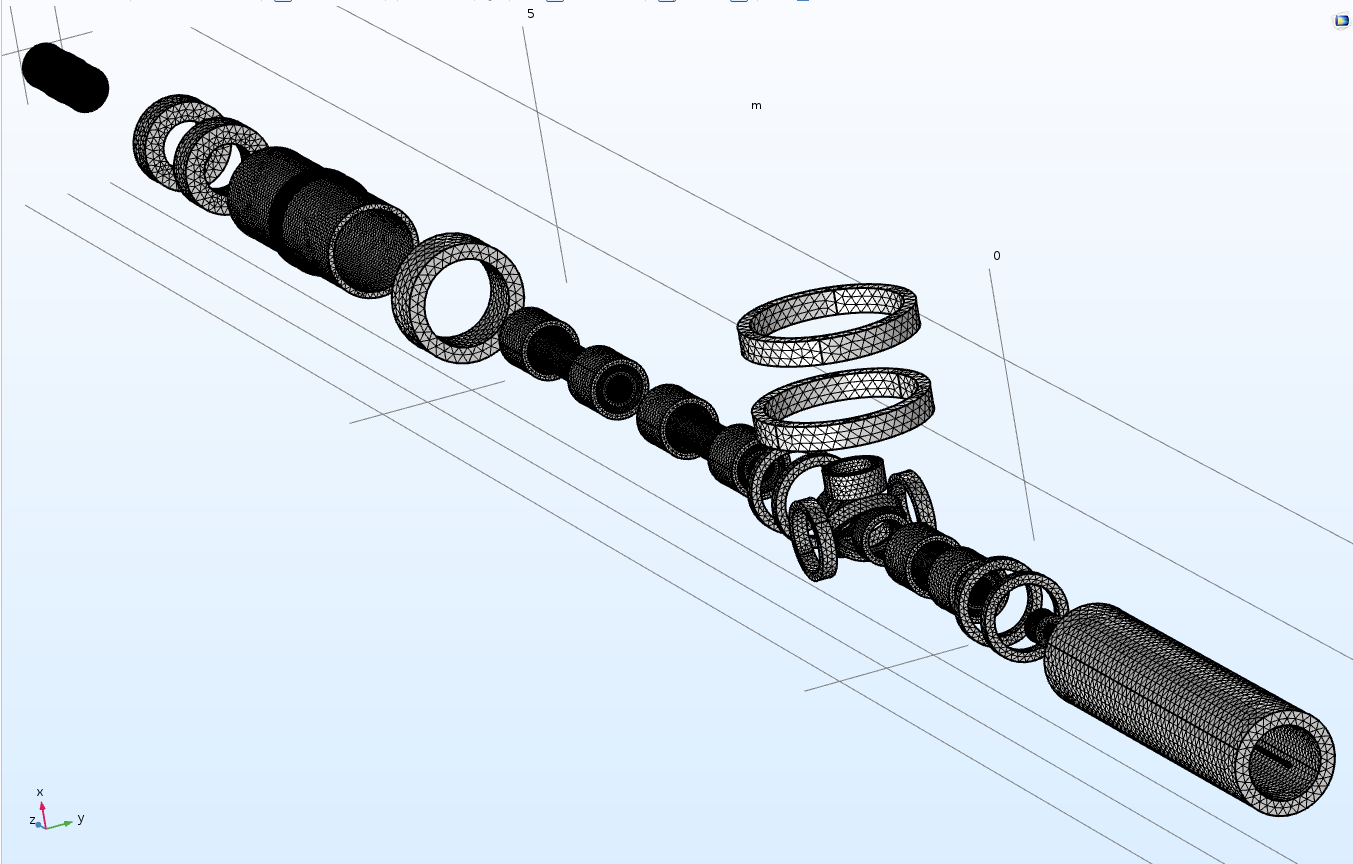
\includegraphics[scale=0.4]{full-mesh}
\caption{Full setup with fine mesh and ready for simulation}
\end{figure}

\subsubsection{Geometry}
To make it possible, we needed to make a 3D model of all of the magnets used in the experiment. The data of magnets was in a file with .cond type which was designed to feed the data to the OPERA software to calculate the magnetic field. After finding the meaning of those numbers on .cond file with the help of my supervisor, First I wrote a python code to transfer those data to a more clear data set of magnets. Then I used the Inventor software to design all of the 82 magnets that were contributing in the magnetic field of the beamline. Then I added the Inventor model of buncher and Accumulator(that was previously created by ALPHA group) to the magnets setup.

\begin{figure}[h]
\centering

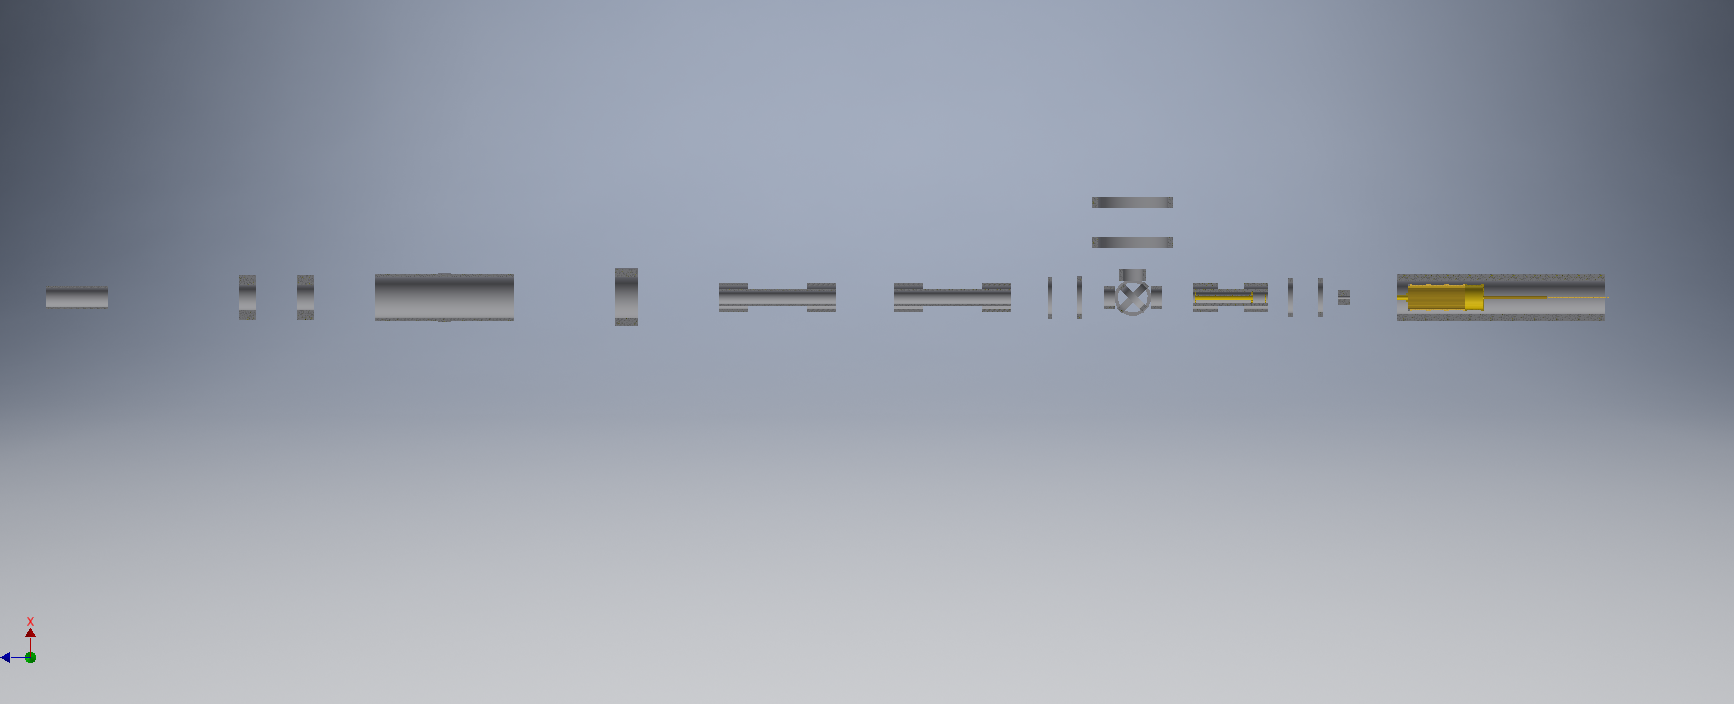
\includegraphics[width=120mm,
height=40mm]{full-beam-line-half}

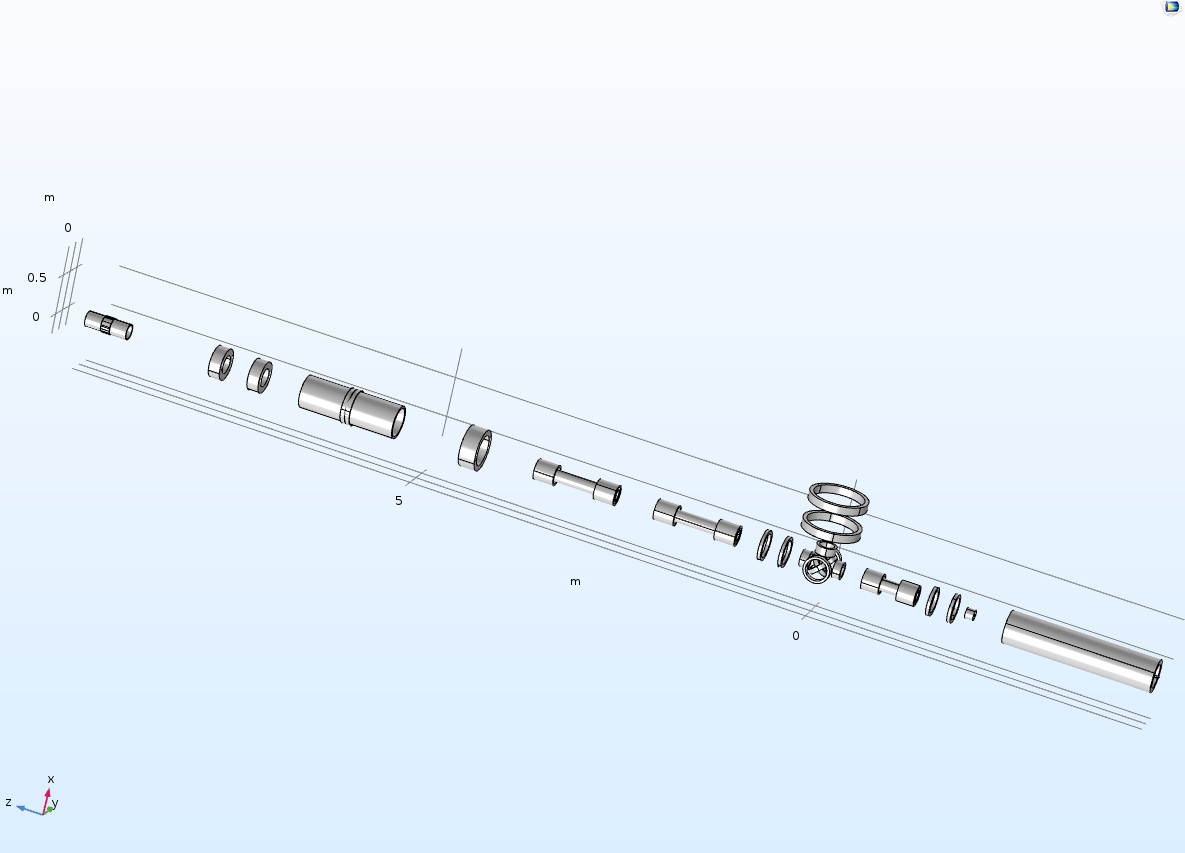
\includegraphics[width=120mm, height=60mm]{full-comsol}
\caption{First: Side view of magnets in Inventor, Second: Model imported to COMSOL environement }
\end{figure}

\subsubsection{Running Simulation on HTCondor Provided by LXPLUS Linux Cluster}
Although I was using two computers in parallel to generate the results faster, simulating the full setup was computationally expensive, So it was impossible to simulate the whole setup with even 32 GB of RAM. The time of simulation was very long as well, so we needed to run our simulation on HTCondor. HTCondor stands for High Throughput Computing and is a specialized workload management system for compute-intensive jobs. Like other full-featured batch systems, HTCondor provides a job queueing mechanism, scheduling policy, priority scheme, resource monitoring, and resource management. Users submit their serial or parallel jobs to HTCondor, HTCondor places them into a queue, chooses when and where to run the jobs based upon a policy, carefully monitors their progress, and ultimately informs the user upon completion(https://research.cs.wisc.edu/htcondor/description.html). Linux clusters of CERN provides the HTCondor and you can access big memory nodes and a higher number of CPU cores. But since I was here at CERN for 53 days, it was impossible to run all of the simulations on clusters and get results. So in this part of my project I created the full simulation file with the real initial values used in apparatus .since I was familiar with Linux I could set up the environment and submit some sample simulations (see figure \ref{cluster}) and my supervisor will run the simulation on cluster after my departure. This simulation contains a parametric sweep to search the optimum values for "amplitude", "Frequency" and "phase" of the sine potential that is applied on the buncher. The real quantitive results will be generated with this simulation and it will help us to tune the parameters of buncher in order to bunch the positron beam.

\begin{figure}[h!]
\centering
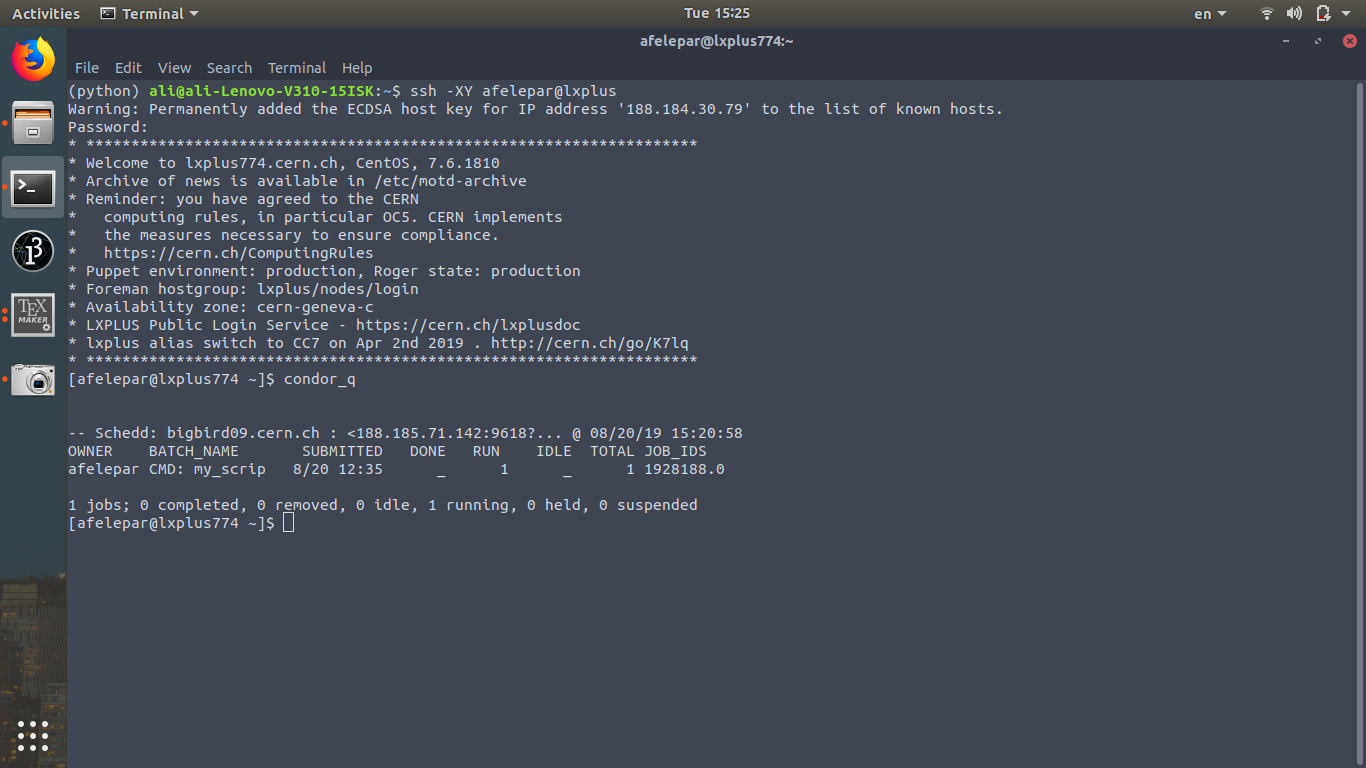
\includegraphics[scale=0.26]{lxplus}
\caption{SSH tunnel to lxplus cluster through linux terminal on my laptop}
\label{cluster}
\end{figure}


\section{Lectures, Workshops and Visits}
During my stay at CERN, I attended almost all of the Lectures. This lecture series was one of the best ones I attended during my life. The content of the lectures was very interesting, the presentation of the lecturers was excellent and the lectures were very up to date. Here is the list of lectures that I attended and the "Physics and Medical Applications" I think was the best among them, and it was the most relevant subject to my field of studies.
\subsection{Classroom Courses}

\begin{enumerate}

\item Physics and Medical Applications by Manjiy Dosanjih
\item Particle World by Tara Shears
\item Detectors by Werner Riegler
\item Foundation of Statistics by Nicolas Berger
\item Electronics DAQ and Trigger
\item Theoretical Concepts in Particle Physics by Andrew Cohen
\item From Raw Data to Physics Results by Paul James
\item Experimental Physics at Hadron Colliders by Marumi Kado
\item The Standard Model
\item Astroparticle Physics
\item Heavy Ions
\item Introduction to Cosmology
\item Beyond Standard Model
\item Nuclear Physics at CERN
\item What is String Theory
\item Future High-Energy Collider Projects
\item Antimatter at Lab

\end{enumerate}


\subsection{Online Courses}
I attendent some Online safety courses which was as following :

\begin{enumerate}
\item Computer Security
\item Emergency Evacualtion
\item Radiation Protection
\item Electrical Safety Fundamentals
\item Electrical Safety Facilities
\item Cryogenic Safety Awarness
\item Chemical Safety Awarness
\end{enumerate}

\subsection{Workshops and Visits}
During the program there was many cool workshops and visits. Here is a list of items that I attended:

\begin{enumerate}

\item Open Data in Educational Activities Workshop
\item Basic Cloud Chamber Workshop
\item Advanced Cloud Chamber Workshop
\item Data Acquistion / Trigger Workshop
\item Root Summer Student Workshop
\item Silicon Senors
\item CMS visit
\end{enumerate} 







\end{document}